%%%%%%%%%%%%%%%%%%% DOCUMENTCLASS BEGIN %%%%%%%%%%%%%%%%%%%
% [onluarkali,tekyonlu],[turkce,ingilizce],[yukseklisans,doktora],
% [bez,karton],[bilisim,fenbilimleri,sosyalbilimler,avrasya,enerji]
% Sample use: \documentclass[onluarkali,ingilizce,yukseklisans,
% karton,fenbilimleri]{itutez}
% Other sample use: \documentclass[tekyonlu,ingilizce,
% yukseklisans,bez,bilisim]{itutez}
% onluarkali: twoside
% tekyonlu: oneside
% turkce: turkish
% ingilizce: english
% yukseklisans: masters
% doktora: phd
% bez: hardcover version
% karton: paperback version
% bilisim: informatics
% fenbilimleri: science and technology
% sosyalbilimler: social sciences
% avrasya: eurasia
% enerji: energy
\documentclass[onluarkali,ingilizce,yukseklisans,bez,fenbilimleri]{thesis}
%%%%%%%%%%%%%%%%%%% DOCUMENTCLASS END %%%%%%%%%%%%%%%%%%%
%%%%%%%%%%%%%%%%%%% TR SETTINGS BEGIN %%%%%%%%%%%%%%%%%%%
%\usepackage[turkish]{babel} % türkçe
%\usepackage[latin5]{inputenc} % latin harfi
%\usepackage[T1]{fontenc} % türkçe heceleme
%\usepackage{fancyhdr}
%%%%%%%%%%%%%%%%%%% TR SETTINGS END %%%%%%%%%%%%%%%%%%%
%%%%%%%%%%%%%%%%%%% PACKAGES & DEFINITIONS BEGIN %%%%%%%%%%%%%%%%%%%
\usepackage{float}
\usepackage[space]{cite}
\usepackage{hyperref}
\usepackage{color}
\usepackage{times}
\usepackage{amssymb,amsmath,mathptmx,amsbsy,bm}
\usepackage{caption}
%\usepackage{floatflt}
%\usepackage[dvipdfm]{graphicx}
\usepackage{graphics}
\usepackage{wrapfig}
\usepackage{epsfig}
\usepackage{enumerate}
\usepackage{rotating}
\usepackage{multirow}
\usepackage{subfigure}
\usepackage{colortbl}
\usepackage{pstricks}
\usepackage{pst-plot}
\usepackage{cite}
\usepackage{latexsym}
\usepackage{rotating}
%\usepackage{subeqn}
%\usepackage{amssymb}
%\usepackage{hyperref}
%\usepackage{url}
%\usepackage{fixltx2e} % Bu paketi sembollerde text ler için subscript yazmakta yardımcı olması için ekliyoruz.
\def\be{\begin{equation}}
\def\ee{\end{equation}}
\def\beq{\begin{eqnarray}}
\def\eeq{\end{eqnarray}}
\def\bse{\begin{subequations}}
\def\ese{\end{subequations}}
\def\nonu{\nonumber}
\def\psibar{\overline{\psi}}

\usepackage{amsmath}
\DeclareMathOperator*{\argmax}{arg\,max}
\DeclareMathOperator*{\argmin}{arg\,min}
\kisaltmalistesi{\hspace{-3mm}

\begin{tabular}{ p{2cm} l }
    {\bf{openCV}} & {\bf:} Open Source Computer Vision Library\\
    {\bf{MLP}} & {\bf:} Milti Layer Perceptron\\
    {\bf{VGG}} & {\bf:} Visual Geometry Group\\
    {\bf{CNN}} & {\bf:} Convolutional Neural Network\\
    {\bf{GAN}} & {\bf:} Generative Adversarial Network\\
    {\bf{PCA}} & {\bf:} Principal Component Analysis\\
    {\bf{GPU}} & {\bf:} Graphics Processing Unit\\
    {\bf{PSNR}} & {\bf:} Peak Signal-to-Noise Ratio\\
    {\bf{SSIM}} & {\bf:} Structural Similarity Index\\
    {\bf{RGB}} & {\bf:} Red, Green, Blue\\
    {\bf{ID-MRF}} & {\bf:} Implicit Diversified Markov Random Fields\\
    {\bf{TV}} & {\bf:} Total Variation\\
    {\bf{ResNet}} & {\bf:} Residual Network\\
    {\bf{MSE}} & {\bf:} Mean Square Error\\
    {\bf{ReLU}} & {\bf:} Rectified Linear Unit\\
    {\bf{FMM}} & {\bf:} Fast Marching Method\\
\end{tabular}

}
\sembollistesi{\hspace{-3mm}
\begin{tabular}{p{2cm}l}
    {\bf{dB}} & {\bf:} Decibel\\
    {\bf{ms}} & {\bf:} Millisecond\\
    {\bf{\(\mu\)s}} & {\bf:} Microsecond\\
    {\bf{ns}} & {\bf:} Nanosecond\\
\end{tabular}}
\onsoz{\setcounter{page}{5}

We would like to thank our adviser, Prof. Dr. Ender Mete Ekşioğlu, for providing guidance and feedback throughout this project.
\newline

January 2021 \newline
\begin{flushright}
\textbf{Halil İbrahim BENGÜ} \\
\textbf{Enes DEMİRAĞ}
\end{flushright}}
\ozet{Görsellerde, bulunulması istenmeyen değişik özelliklere sahip bölümler bulunabilmektedir. Bu bölümler eğer söz konusu görsel, fiziksel olarak bulunan bir görsel ise görselin eskimesi sebebiyle oluşmuş olabileceği gibi, dijital bir resimde istenmeyen bir obje veya bölge de olabilir. Görsellerden bu hataların düzeltilmesi veya bu bölümlerin görsellerden çıkartılıp, yerlerinin gerçekçi bir şekilde doldurulmak istenmesi günümüzde araştırma alanı olduğu gibi aynı zamanda ticari bir problemdir. Bu amaca yönelik çok sayıda özelleşmiş araçlar bulunmaktadır ve bu araçların kullanılması profesyonel kullanım da gerektirebilmektedir.

Derin Öğrenme ile Resim Boyama projesinde amaç, resimlerde bulunan ve görsellerden çıkarılan bu bölgeleri dolduran farklı yapıların incelenmesidir. Bu amaç doğrultusunda, bir çok farklı proje, türlerine göre gruplara ayrılmış ve bu gruplardan örnek çalışmalar karşılaştırılmıştır. İncelenmek üzere inpainting yöntemleri geleneksel yöntemler ve derin yöntemler olmak üzere ikiye ayrılmıştır. Çalışmamız sırasında fazla sayıda yöntemden bahsedilmiş olmakla birlikte, karşılaştırma için geleneksel yöntemlerden navier-strokes ve fast-marching yöntemleri seçilmiştir. Derin yöntemler arasından da başarılı sonuçlar verdiği tespit edilen, EdgeConnect, Generative Contextual, Generative Multi-column Convolutional Neural Network ve Deep Image Prior yöntemleri detaylı olarak incelenmek ve gerçeklemek üzere seçilmiştir. Bütün bunlara ek olarak, çalışmamızın sonunda incelemiş olduğumuz farklı tür çalışmalardan ilham alarak gerçeklemeye karar verdiğimiz 2 yöntem de incelenmiş ve görsel sonuçlar elde edilmiştir.

Derin yöntemlere örnek olarak seçtiğimiz iki yöntemimiz EdgeConnect ve Generative Contextual, GAN adı verilen ve birbirlerine zıt çalışan iki derin yapay sinir ağı temelli çalışmalardır. EdgeConnect çalışmasında iki aşama bulunmaktadır ve bu iki aşama da bahsedilen GAN yapısını kullanmaktadır. Birinci aşamada girdi olarak alınan görselin eksik bölgelerindeki sınır çizgileri tahmin edilmeye çalışılmakta, ikinci aşamada oluşturulan sınır çizgileri ve maskelenmiş görsel kullanılarak eksik bölgesi doldurulmuş görsel üretilmek istenmektedir. Generative Contextual çalışmasında da GAN kullanan 2 aşama bulunmaktadır. İlk aşamada kabaca maskelenmiş bölge doldurulmakta, ikinci aşamada ise oluşturulan görsel üzerinde, anlam bilgisi elde etmeyi amaçlayan bir katman da kullanılarak iyileştirme çalışmaları yapılmaktadır.

Seçilmiş olan diğer bir derin resim boyama çalışması ise konvolusyon katmanlarını paralel olarak kullanan Generative Multi-column CNN yöntemidir. Bu yöntem girdi olarak aldığı görseli farklı boyutlarda filtreler kullanarak paralel CNN yapılarından geçirir. Ardından görsel üzerindeki farklı seviyede bilgi elde etmeyi sağlayan bu yapılar bir araya getirilir ve sonuç olarak resim boyama işlemi tamamlanmış olur.

Son olarak ayrıntılı incelediğimiz bir diğer yöntem ise Deep Image Prior yöntemidir. Bu yöntem herhangi bir dataset kullanılarak bir model eğitilmesi ihtiyacı olmadan resim boyama işlemini gerçekleştiren bir yöntemdir. Resim boyama dışında süper-çözünürlük ve gürültü giderme gibi uygulamalarda da kullanılabilen bu yöntem çeşitli CNN yapılarını kullanarak iteratif olarak sonuç elde eder. 

Çalışmamız sırasında Pytorch ve Tensorflow derin öğrenme kütüphaneleri kullanılmıştır. Özellikle derin yöntemlerin eğitilmesi ve test aşaması için ciddi işlem gücü gerekmesi sebebiyle çalışmalarımız ekran kartı üzerinde çalıştırılmıştır. Çalışmalarımızın sonucunda, testlerini gerçeklediğimiz farklı çalışmalar örnek görsellerle birlikte, PSNR ve SSIM değerleri üzerinden karşılaştırılmış ve sunulmuştur.}
\summary{There may be parts in the images with different features that are not desired. These undesired parts might be caused by aging of a photograph or these parts could include an object which is wanted to be removed from the image. Removing these parts and inpainting them with visually realistic features is both a research area and a commercial problem. There are many specialized tools for this purpose and use of these tools may also require professional knowledge.

The aim of the Image Inpainting with Deep Learning project is to examine the different structures in the pictures that fill these regions that are extracted from the pictures. For this purpose, many different work types were divided into groups and sample studies from these groups were compared. Inpainting methods for review purposes, are divided into two as traditional methods and deep methods. Although many methods were mentioned during our study only a few are chosen. Navier-strokes and fast-marching methods were chosen for comparison as example of traditional methods. EdgeConnect, Generative Contextual, GMCNN (ASIL ADI) and Deep Prior methods, which were found to give successful results among deep methods, were selected to be examined in detaial and implemented. In addition to all these, two novel methods are implemented which are inspired from all methods we examined throughout this project. Results of these two methods are also explained and examined in this project.

As examples of deep methods, our two methods, EdgeConnect and Generative Contextual are two GAN based studies which use deep artificial neural networks that work adversarial to each other. There are two stages in the EdgeConnect method and these two stages use the mentioned GAN structure. In the first stage, corrupted image is taken as input to the model and edge information is predicted, and in the second stage, it is desired to produce an image whose missing region is filled by using the both edge information and masked image. Also, in Generative Contextual study there are two stages that use GAN aswell. In the first stage, maske area is inpainted roughlt, and in the second stage, improvement operations are carried out on the created image by using a layer that aims to obtain contextual information.

% CNN Part

Pytorch and Tensorflow artificial intelligence libraries were used during our study. Our studies were run on the graphics card, especially since serious processing power was required for training and testing of deep learning methods. As a result of our project, different studies that we tested were compared and presented with PSNR and SSIM values and example images.}
\ozgecmis{\vspace{10mm}

\newsavebox{\mysquare}
\savebox{\mysquare}{\textcolor{black}{\rule[2.3pt]{3.4pt}{3.4pt}}}

\setlength{\TPHorizModule}{10pt}
\setlength{\TPVertModule}{10pt}
\begin{textblock}{1}(40,17)
  \begin{figure}[p]
    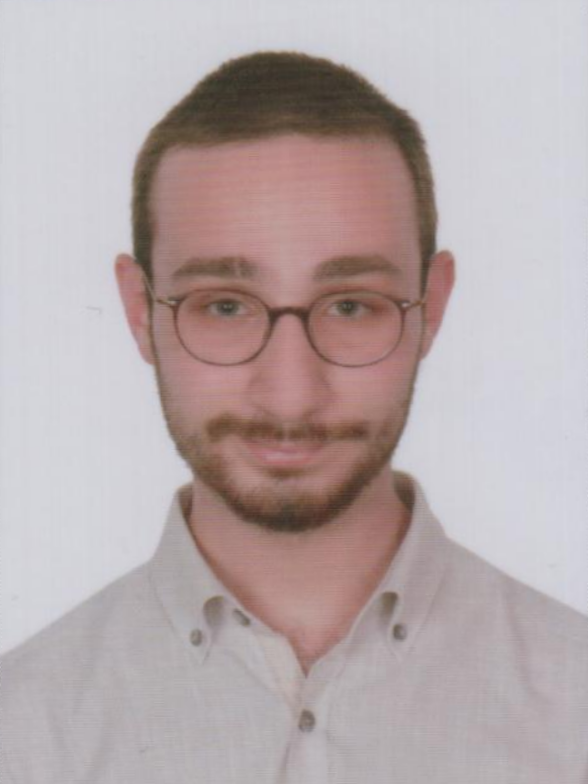
\includegraphics[scale=0.25,keepaspectratio=true]{figures/vesikalik-enes.png}
    % photo.eps: 0x0 pixel, 300dpi, 0.00x0.00 cm, bb=14 14 279 359
  \end{figure}

\end{textblock}
\textbf{Name Surname: {\normalfont Enes Demirağ}} \\

\vspace{-3mm}
\textbf{Place and Date of Birth: {\normalfont Istanbul, 28/05/1998}} \\

\vspace{-3mm}
\textbf{E-Mail: {\normalfont demirag16@itu.edu.tr}} \\


\textbf{EDUCATION:}
\vspace{-3mm}
\begin{itemize}
  \item \textbf{B.Eng.:} 2016 - 2021, Istanbul Technical University, Faculty of Electrical and Electronics Engineering, Electronics and Communication Engineering
  \item \textbf{Erasmus Program:} Jan. - June 2019, Liverpool John Moores University, UK
\end{itemize}

\textbf{PROFESSIONAL EXPERIENCE AND REWARDS:}
\vspace{-3mm}
\begin{itemize}
  \item Baykar Technologies \hfill \textit{Aug 2020 - Present}
  \item Ravinspect Tech \hfill \textit{July 2018 - Sept. 2018}
  \item DESI Security \& Lock Systems \hfill \textit{July 2017 - Aug. 2017}
  \item ITU Department of Information Technology \hfill \textit{Apr. 2017 - July 2017}
\end{itemize}


\vspace{-3mm}

\newpage

\vspace{10mm}

\newsavebox{\mysquarebeng}
\savebox{\mysquarebeng}{\textcolor{black}{\rule[2.3pt]{3.4pt}{3.4pt}}}

\setlength{\TPHorizModule}{10pt}
\setlength{\TPVertModule}{10pt}

\begin{textblock}{1}(40,17)
  \begin{figure}[p]
    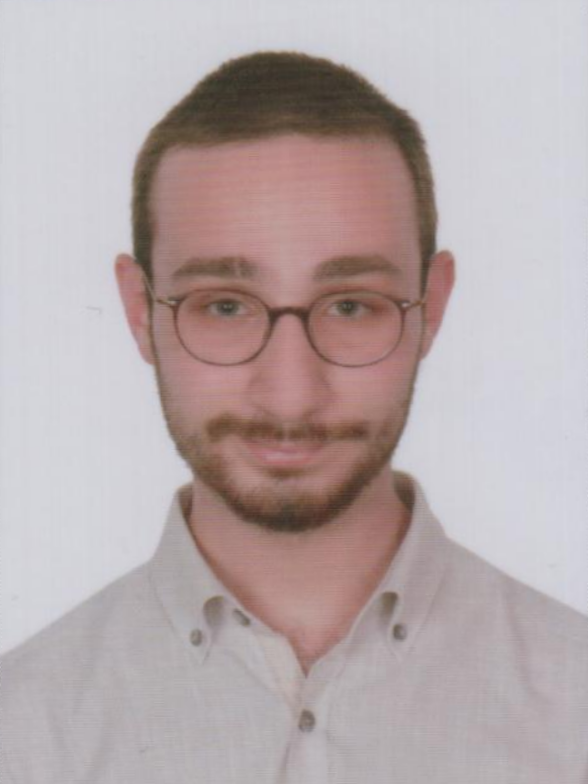
\includegraphics[scale=0.25,keepaspectratio=true]{figures/vesikalik-enes.png}
    % photo.eps: 0x0 pixel, 300dpi, 0.00x0.00 cm, bb=14 14 279 359
  \end{figure}

\end{textblock}
\textbf{Name Surname: {\normalfont Halil İbrahim Bengü}} \\

\vspace{-3mm}
\textbf{Place and Date of Birth: {\normalfont Istanbul, 27/04/1998}} \\

\vspace{-3mm}
\textbf{E-Mail: {\normalfont bengu16@itu.edu.tr}} \\


\textbf{EDUCATION:}
\vspace{-3mm}
\begin{itemize}
  \item \textbf{B.Eng.:} 2016 - 2021, Istanbul Technical University, Faculty of Electrical and Electronics Engineering, Electronics and Communication Engineering
  \item \textbf{Erasmus Program:} Jan. - June 2019, Linköping University, SWE
\end{itemize}

\textbf{PROFESSIONAL EXPERIENCE AND REWARDS:}
\vspace{-3mm}
\begin{itemize}
  \item Pavelsis \hfill \textit{Nov. 2020 - Present}
  \item Aselsan \hfill \textit{July 2020 - Sep. 2020}
  \item Kaizen Telecommunication \hfill \textit{July 2018 - Sep. 2018}
\end{itemize}


\vspace{-3mm}
% ---------------------------------------------------------------- %
% Fotografli ve yayin listeli (yayini varsa) ozgecmis onerilir.    %
% Fotograf ve adres sart degildir.				   %
% ---------------------------------------------------------------- %
}
%%%%%%%%%%%%%%%%%%% PACKAGES & DEFINITIONS END %%%%%%%%%%%%%%%%%%%
%%%%%%%%%%%%%%%%%%% DOCUMENT BEGIN %%%%%%%%%%%%%%%%%%%
\begin{document}
%%%%%%%%%%%%%%%%%%% CHAPTERS BEGIN %%%%%%%%%%%%%%%%%%%
\chapter{INTRODUCTION}\label{introduction}

\pagenumbering{arabic}

Inpainting is the process of reconstructing missing and corrupted regions in an image. Early works in this field started with manually repairing deformed photographs by a talented artists. With the transition from analog photography to digital images, algorithms that can perform this process in a much shorter time started to appear. With the development of deep learning technologies and the increase in image data resources, the use of artificial neural network models has become more popular to solve this problem. These methods perform the image inpainting process completely automatically without the need for people.

Image inpainting can be used for purposes such as removing an unwanted object from the image or restoring a noisy image by filling the missing data in images. Traditional image restoration methods are basically designed to fill missing pixel values in a way that similar to the neighboring pixel values. These methods usually give poor results in cases with large missing areas.

Modern methods are usually trained with millions of images from thousands of different labels using supervised machine learning. For example, generative adversarial network, which has the ability to generate new data, is frequently used in such studies. A neural network alone cannot understand the places that need to be filled in an given input image. Therefore, input image is given along with a mask indicating that the related corrupted parts in the image are missing and need to be filled. Then, output image is generated by passing through various network layers. The missing parts of the original image are filled by taking the masked parts from this generated output image.
\chapter{TRADITIONAL METHODS}\label{traditional_methods}

There are many different methods used for image inpainting. Each of these methods has mathematical foundations in itself. These methods are categorized according to methods they use to get the desired output\cite{exemplerinpainting}. The first of these methods are the methods called traditional methods that try to correct the missing part on the main title picture only with the features in the picture to be corrected.

Machine learning methods, which have been used frequently in many different problems due to increased processing power and broad access to large data sets, have also started to be used for image inpainting problems. These ideas, which will be explained under the title of traditional methods, also formed the basis for machine learning and deep learning methods used for inpainting. The methods explained under this title were used in different deep learning methods, which will be examined later.

It would be more accurate to examine traditional methods mainly as exemplar-based and diffusion based. Although Exemplar-based methods are divided into pixel-based and patch-based, patch-based methods will be examined mainly in exemplar-based methods, since there are more studies relating to patch-based methods and they give better results. \cite{trad1} and \cite{trad2} are some of the traditional method example works.

As can be understood from their names, patch-based methods try to fill the missing region in the picture with the information obtained from different parts of the picture. Diffusion-based methods try to fill the region by diffusing surrounding pixels from its boundary \cite{navier_stokes_inpainting}, \cite{telea}.

Traditional methods are methods that do not require training. For this reason, it is an appropriate method to use for simpler problems. Traditional methods do not work well in problems where the masked area in the picture starts to form a proportionally large area. This result is quite normal given that these methods infer from pixels near the missing region.

\section{Patch-based Methods}

Patch-based image inpainting consists of methods that use the undamaged regions in the image to create the region to be filled. With this approach it is aimed to have the highest possible patch similarity level\cite{inpaintingoverview}.

In order to implement this method, an algorithm is needed on how to transfer the obtained regions to the areas planned to be filled. Another important point in this method is the selection of the algorithm that will compare the regions in different parts of the picture with the regions desired to be created \cite{patchmatch}.

While patch-based methods work well, they assume that the information in the missing part of the picture resides elsewhere in the picture. Another problem with patch-based methods is that they require relatively more processing power because they are methods that consistently involve searching and comparing.

\subsection{Patch-based Texture Synthesis}

In this method by Zhou et al \cite{patch_based_tex_synthesis}, it is aimed to fill the desired area by creating textures with patch-based algorithms for Image inpainting method. While implementing this targeted method, a road starting from the rough, proceeding in detail is aimed. While performing the filling process, targets and constraints were created in order to ensure the integrity of the newly created region with the rest of the picture.

In this study, a more efficient inpainting study has been achieved by basically using the successive elimination algorithm and based on the previously used methods.

Texture synthesis is performed by trying to imitate information about texture and structure integrity. At the same time, it is aimed to reduce the processing power used by using the successive elimination algorithm during texture comparison.

In this approach, the function given in equation \ref{eqn:textsynth} is tried to be minimized in order to achieve the desired result.

\begin{equation}
    \label{eqn:textsynth}
    I_t = \frac{1}{k_p} \displaystyle\sum\limits_{q\epsilon\Omega} {I_qf(|p-q|).g(|I_p-I_q|)}
\end{equation}

However, minimizing this equation does not mean that the energy function decreases in general. To explain better, the region to be filled in the image can be completely filled with a smaller patch than itself and gives a perfect result in the equation. However, for better results, coarse images as  are used in equation \ref{eqn:textsynth2} and equation \ref{eqn:textsynth3}.

\begin{equation}
    \label{eqn:textsynth2}
    \lambda(x,y)(\mu_1-\mu_0)=\mu\Delta^2\mu1, where \frac{\partial\mu_1}{\partial n}
\end{equation}

\begin{equation}
    \label{eqn:textsynth3}
    \lambda(x,y)(\mu_2-\mu_0)=\mu\Delta^2\mu2, where \frac{\partial\mu_2}{\partial n}
\end{equation}

In this way, the image inpainting process for the visual is corrected to give a good result from the rough approach. However, this process requires a high processing power due to 3 different partial differential equations.

\begin{equation}
    \label{eqn:textsynth4}
    E(c_k, C) = \sum\limits_{k}\int\limits_{\Omega_k}\lambda(x,y){(c_k,\mu_0)}^2dxy+V|C|
\end{equation}

It is logical to use an approach to solve this problem. With this approach, uniform visual densities can be accepted as constant for different regions. Hence, MS energy function can be reduced to equation \ref{eqn:textsynth4}. Also, an inpainted image example with its input image is given in figure \ref{fig:patch-based-example}.

\begin{figure}[h]
    \centering
    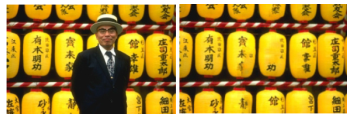
\includegraphics{figures/chapter2/Patch-Based-texture-synth-example.png}
    \vspace*{5mm}
    \caption{Inpainted Image with Patch Based Texture Synthesis\cite{patch_based_tex_synthesis}}
    \label{fig:patch-based-example}
\end{figure}

\subsection{Image Melding}

The image melting method \cite{imagemelding} creates a transition zone to transfer various information and properties within one image to another image. This method can be used for different purposes depending on the usage type.

This method, primarily uses many different transforms to increase the ability to search for patches. Next, image gradients are included in patch representation and Poisson equation solver is used for color averaging. Without causing blurry areas in the picture, a new energy method is used based on \(L_2/L_0\) norms for colors. Melding of 2 different image is illustrated below in figure \ref{fig:image-melding-example}.

\begin{figure}[h]
    \centering
    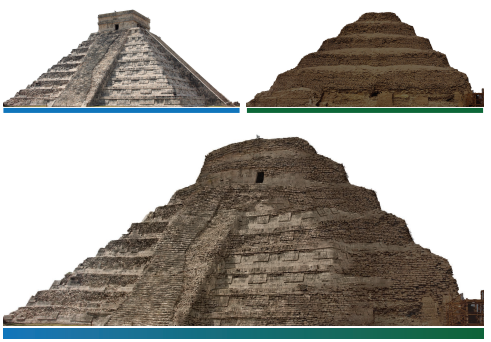
\includegraphics{figures/chapter2/Image-Melding.png}
    \vspace*{5mm}
    \caption{Image Melding Example \cite{imagemelding}}
    \label{fig:image-melding-example}
\end{figure}

Many different patch-based methods have been used for inpainting problems. Image melding is basically a patch-based algorithm. However, when based-patched methods are given inconsistent visuals, they can give insufficient results because they use a direct distance function between pixels.

Another result aimed with this study is that patch-based and gradient methods can be used together and thus more complex problems can be solved. Thanks to the methods used, Image Melding can be used to solve many different problems including inpainting.

Image synthesis using a single source is one of the ways image melding can be used. In this algorithm, a mask divides the image into two parts, S and T, respectively, as source and target. After this process, the energy function shown in equation \ref{eqn:imagemelding1} is obtained.

\begin{equation}
    \label{eqn:imagemelding1}
    E(T,S) = \sum\limits_{q\subset T}{min_{p\subset S}(D(Q,P)+\lambda D(\Delta Q, \Delta P))}
\end{equation}

In the above equation Q represents the targeted patch with w width and height and target pixel q on the upper left corner. P represents the transformation that is applied to the neighbor pixels of the source pixel. Throughout the operations, all patches have 5 channels, which 3 of them are RGB and 2 channels are gradient channels. In the equation \ref{eqn:imagemelding1}, RGB channels are shown with Q and P, gradient channels are shown with \(\Delta Q \Delta P \)Distances for all channels are expressed with D and,  weight the gradient channels in according to RGB channels.

Two important steps during the implementation of the algorithm are searching and voting. For the search part, the PatchMatch algorithm is properly used. With using this algorithm, patches with sufficient proximity are detected for the target patch. Translation, rotation and scaling are used freely during this process. At the same time, ranges are defined on the channels in order to obtain better results.

\begin{equation}
    \label{eqn:imagemelding2}
    T= argmin(D(I,\bar{T}+\lambda D(\Delta I,\Delta \bar{T}))
    %sYanlislik olabilir mi kontrol et bir ara
\end{equation}

In the Voting part, an algorithm is used in which every pixel in the patch is included, and the resulting output takes its form in eq \ref{eqn:imagemelding2}. In figure \ref{fig:inpainting-image-melding}, Inpainting example with image melding method is given.

\begin{figure}[h]
    \centering
    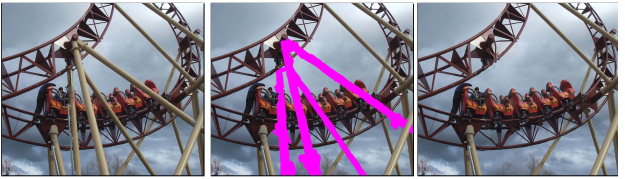
\includegraphics{figures/chapter2/ImageMeldingExample.png}
    \vspace*{5mm}
    \caption{Inpaingting Example with Image Melding\cite{imagemelding}}
    \label{fig:inpainting-image-melding}
\end{figure}

\section{Diffusion-based Methods}

This method basically fills missing regions or unwanted objects in an image by diffusing neighboring pixel information. Diffusion process uses partial differential equations. Inpainting is not the only use of such diffusion-based methods. In addition, these type of methods are available in areas like image compression. Diffusion-based image inpainting can be used to remove undesirable objects in an image or to repair damaged parts of it. However, as a downside, these methods can leave artifacts after inpainting process such as local variance difference and noise pattern \cite{diffusion_based_artifacts}. In figure \ref{fig:diffusion_based_inpainting} an example of diffusion-based inpainting can be seen. The black region in \ref{fig:diffusion_based_inpainting}.a is the unknown region and the \ref{fig:diffusion_based_inpainting}.b shows the inpainting result, the region surrounded by the dashed curve is recovered by inpainting.

Basically, the inpainting process is nothing more than restoring the missing pixel information in an image and there are some common assumptions that most of the images have commonly share. In this way of thinking, Navier-Stokes based method \cite{navier_stokes} was introduced. Navier-Stokes equations known in the area of mechanics, especially fluid mechanics. This inpainting method emerged by combining ideas in the field of classical fluid dynamics with the help of partial equations and remains one of the most popular traditional methods to this day. The assumption that the edges in an image are contunious is used. The authors designed this inpainting method by considering the color information of the surrounding pixels and the this continuity constraint.

\begin{figure}[h]
    \centering
    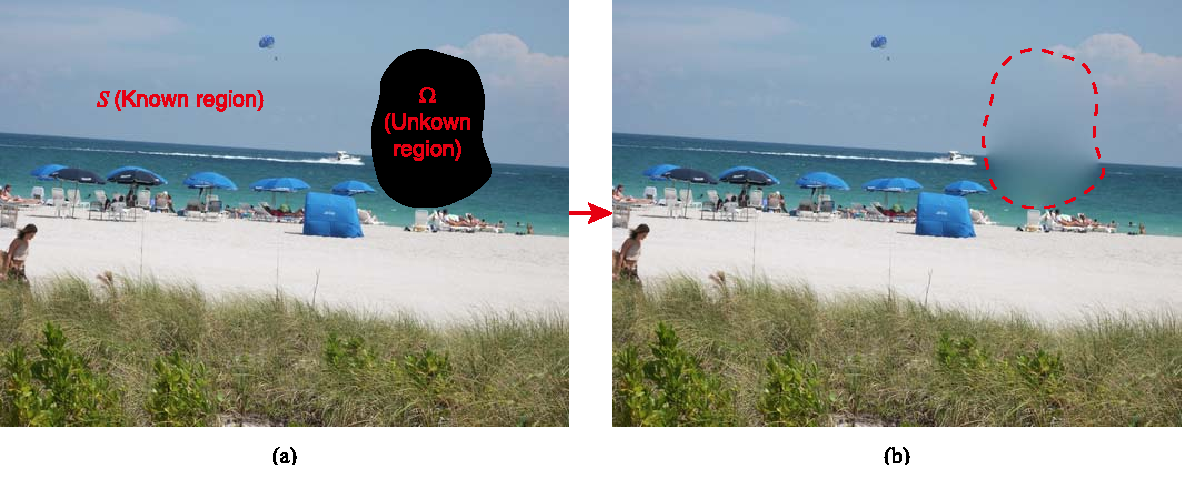
\includegraphics[width=14cm]{figures/chapter2/diffusion_based_inpainting.png}
    \caption{Diffusion-based inpainting example \cite{diffusion_based_inpainting}}
    \label{fig:diffusion_based_inpainting}
\end{figure}

Another traditional inpainting study based on fast marching method \cite{telea} proposed that, in order to estimate the color of the missing pixels, gradients of the neighbor regions can be used. In our work, these two methods used as a baseline when comparing the deep learning based inpainting methods with traditional inpainting methods.

\subsection{Navier-Stokes Method}

Navier-Strokes equations are partial differential equations for describing the motion of fluid substances. These equations used in variety of areas in different industries such as modeling ocean currents, weather conditions and even when designing aircrafts and cars.

\begin{equation}
    \omega_{t} + \upsilon \cdot \nabla \omega = \nu \nabla \cdot \left ( g \left ( \left | \nabla \omega \right | \right ) \nabla \omega \right)
    \label{eq:navier_stokes}
\end{equation}

In this method \cite{navier_stokes}, the stream function formulation used in fluid mechanics has been made suitable for the inpainting process. The counterpart to the vorticity-stream function for inpainting transform into equation \ref{eq:navier_stokes} which corresponds to the solution of the intensity value of a pixel. \cite{navier_stokes_inpainting} Similarly, the fluid velocity in fluid dynamics corresponds to the gradient of the intensity values also interpereted as isophote direction, vortocity corresponds to smoothness and viscosity corresponds to diffusion respectively in this problem.

The algorithm used in this study proceeds by following the edges in the picture from the known region to the unknown region. Since it is assumed that the edges will be continous during this progress, isophote lines are preserved. Isophote means the lines created by pixels with the same intensity value. During this process, the direction of the gradient vector in the boundaries preserved. After the isophotes are obtained, color information is calculated to reduce the minimum variance and by filling in the unknown pixels, the inpainting process is completed.

\subsection{Fast Marching Method}

In this study published in 2004 \cite{telea}, Ahmet developed an inpainting technique based on the fast marching method. A filling process is designed starting from the boundary pixels of a region where the pixel information is missing and going step by step towards the inside. It takes a small neighborhood of pixels to calculate the unknown pixel value as the weighted sum of known pixels inside that boundary. For this weighted summation process, the weights selected according to the proximity and boundary normal. After all the pixels are calculated in each step, the next closest pixel is passed with the fast marching method and the same process is repeated again until everything inside the region is inpainted. FMM ensures that the pixels which are near to the known pixels inpainted first and inside pixels will be filled afterwards. This inpainting priciple can be seen in figure \ref{fig:ffm}. Pixel \(p\) in figure \ref{fig:ffm}.a will be inpainted. Inside a small region \(\epsilon\), for any \(q\) known pixel, the gradient \(\nabla I\) will be calculated as seen in figure \ref{fig:ffm}.b.  

\begin{figure}[h]
    \centering
    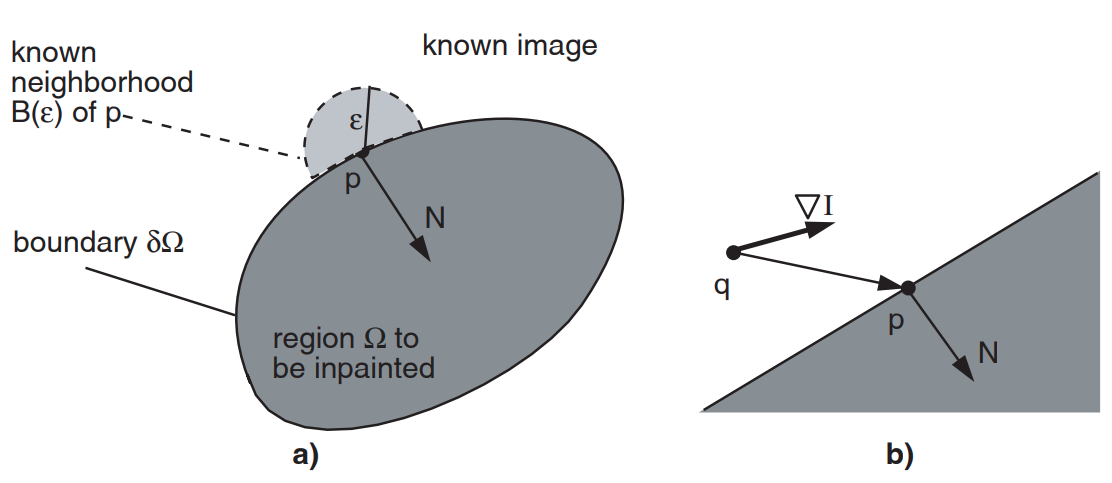
\includegraphics[width=14cm]{figures/chapter2/ffm.png}
    \vspace*{4mm}
    \caption{Fast marching method inpainting priciple}
    \label{fig:ffm}
\end{figure}

In figure \ref{fig:traditional_comparison}, comparison of the Navier-Stokes and Fast Marching approaches can bee seen. White colored pixels in \ref{fig:traditional_comparison}.a are the missing areas and \ref{fig:traditional_comparison}.d is the original image. In \ref{fig:traditional_comparison}.b, output of the Navier-Stokes method and in \ref{fig:traditional_comparison}.c, output of the Fast Marching method shown respectively.

\begin{figure}[h]
    \centering
    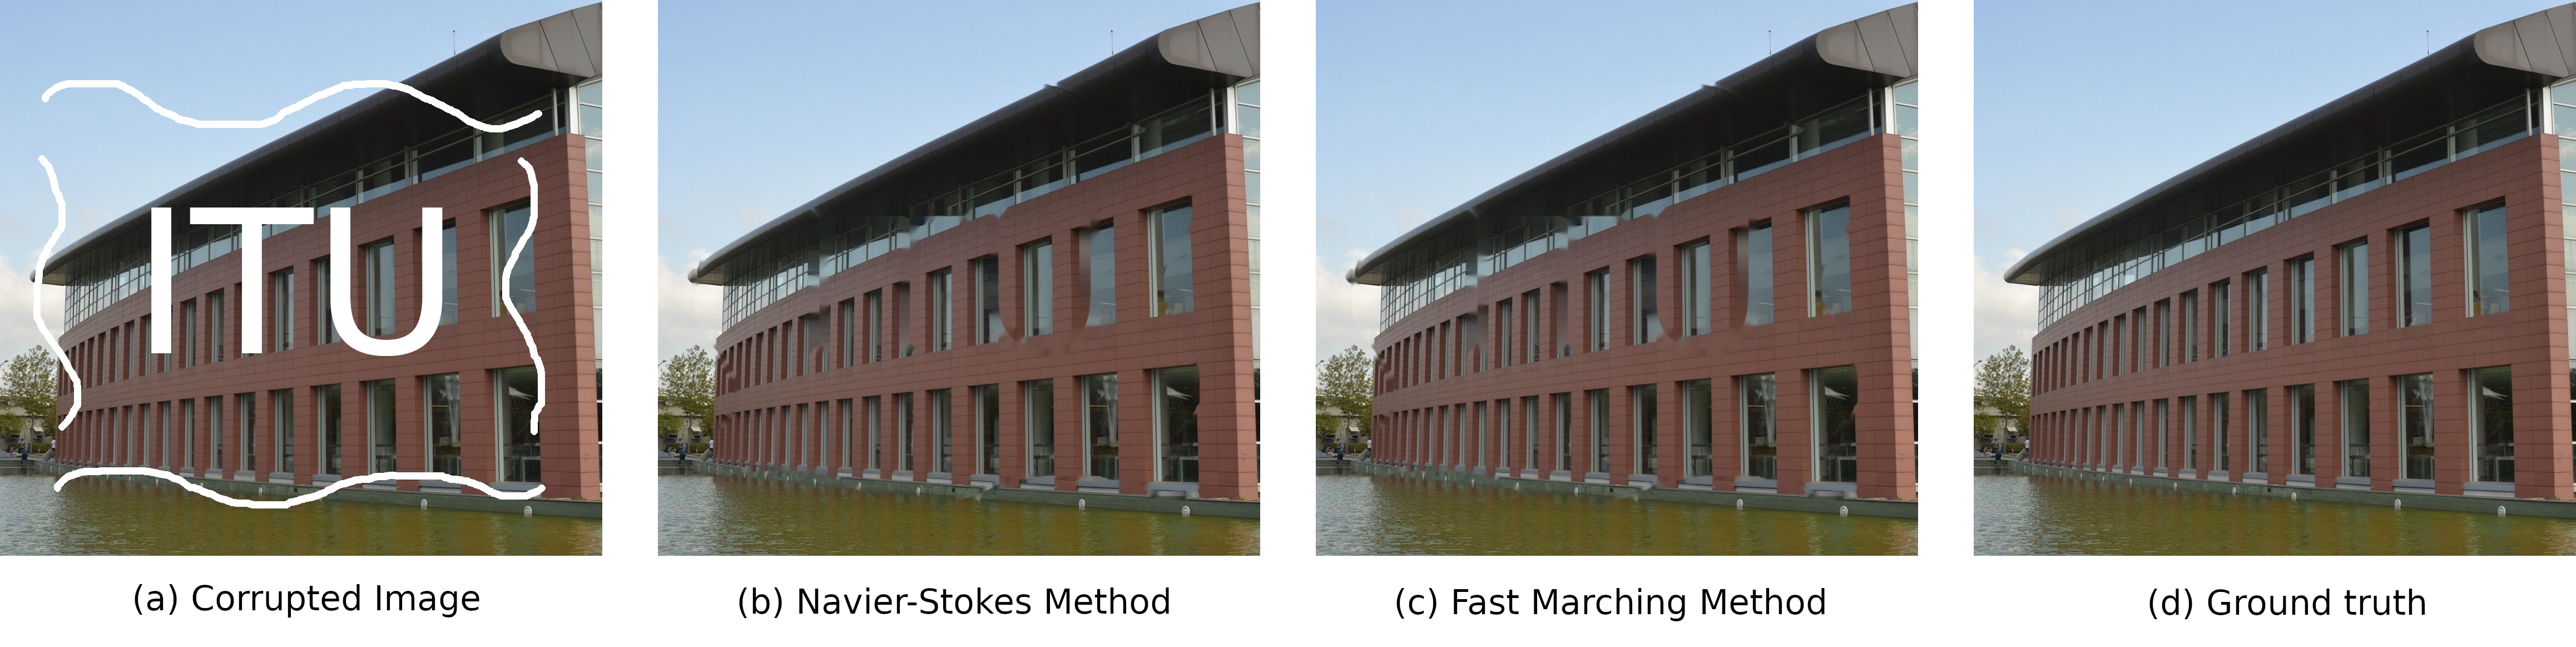
\includegraphics[width=14cm]{figures/chapter2/traditional_comparison.png}
    \caption{Comparison of Navier-Stokes and Fast Marching methods}
    \label{fig:traditional_comparison}
\end{figure}

\chapter{INTRODUCTION TO MACHINE LEARNING}\label{intro_to_ml}

\section{Machine Learning}

Machine learning is the modeling of complex systems on mathematical and statistical operations that perform tasks such as regression, classification and clustering using data. Thus, with the help of these algorithms computers can perceive mixed patterns in data. Today, there are many different machine learning methods for variety of data types. These learning methods are generally divided into three categories. These categories are supervised learning, unsupervised learning and reinforcement learning respectively. Supervised learning methods use training data with corresponding labels which defined beforehand. Label also known as ground truth represents the expected output of the machine learning system. This type of learning algorithms try to come up with a mapping function between training data and the ground truth. As an example, speech recognition \cite{speech_recognition} or a regression problem such as market forecasting \cite{market} can be solved using this type of learning. The second category is the methods implemented using only data without any corresponding ground truth. Two example of the areas of use of such unsupervised learning algorithms are the clustering problem in the recommender systems \cite{recommender_systems} and the dimension reduction \cite{pca}. The last category, reinforcement learning, is used in solving problems that require real-time decision making. For example, in the field of robotics, the methods under this category are used in the design of the systems to decide what action to take against any state in an environment \cite{robotics}.

Deep learning is a subclass of the much broader area of machine learning applications. In order to comprehend the methods mentioned in this thesis well, it is necessary to have a knowledge of statistics, calculus, optimization and computer vision as well as machine learning basics. For this reason, some machine learning basics are mentioned in the following chapters.

\section{Neural Networks}

The idea of a neural networks are although they could not be realized efficiently for a long time, is an idea in machine learning field that emerged more than 70 years ago, and represents a similarity to neurons in the human brain. First neural network is created by McCulloch and Pitts, however they did not have enough technology to run it. Later in 1954, Clark and Farley at MIT were able to run the first Neural Network.

The main feature that enables neural networks to work is that they are made of neurons. These neurons are similar to neurons in the human brain. The basic requirement for understanding how neural networks work is to understand how neurons in the human brain work and how it connects to Artificial Neural Networks (ANN).

There are billions of neurons in a human brain. These neurons communicate with each other using electrical signals. Neurons produce their own output according to the different types of signals they receive. If the value they receive is above a certain limit, it generates electrical impulse in response.

As with a real neuron, a neuron in the ANN also functions similarly. The neurons in the ANN simply take the input they receive and process this data and then give an output. Each neuron in the network has its own parameters called weights. This decision-making process produces an output yes or no. Hence, it is possible to call this process a classifier. Similar to a neuron function, a threshold function is illustrated in figure \ref{fig:threshold}.

\begin{figure}[h!]
    \centering
    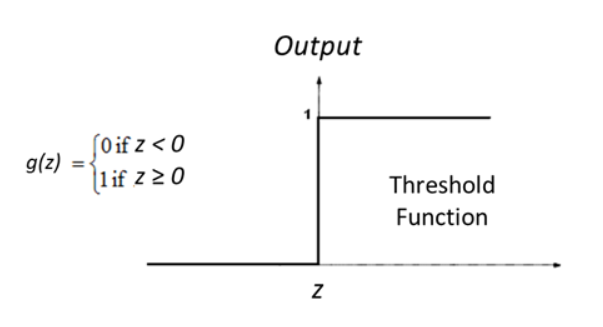
\includegraphics[scale=0.7]{figures/chapter3/threshol.png}
    \caption{Threshold Function}
    \label{fig:threshold}
\end{figure}

There are different numbers of layers in ANN depending on their size. Neurons transmit their output from each layer to the next layer. As will be explained later, the output from each neuron is inserted into activation functions to ensure non-linearity within the system. Neuron structure is shown in figure \ref{fig:neuron_drawl}.

\begin{figure}[h!]
    \centering
    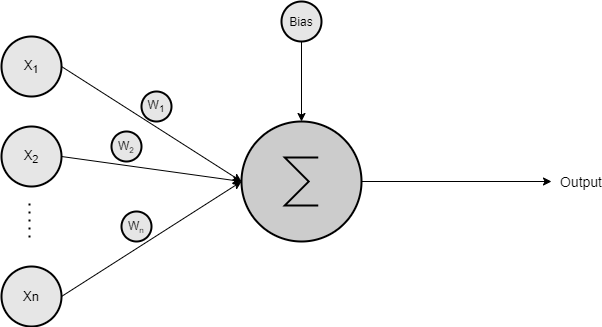
\includegraphics[scale=0.5]{figures/chapter3/neuron.png}
    \caption{Neuron}
    \label{fig:neuron_drawl}
\end{figure}

Based on the ideas previously announced, McCulloch and Pitts designed the first neural network. In the system they designed, many inputs are given to each neuron as input, and the output of the neuron can be obtained by adding these inputs after multiplying with weights. The output of this neuron is also directed to the activation function.Operations done in a neuron are shown in \ref{eqn:nn1} and \ref{eqn:nn2}.

\begin{equation}
\label{eqn:nn1}
    Out = \sum\limits_{i=1}^{N}{I_i W_i}
\end{equation}

\begin{equation}
\label{eqn:nn2}
    Y = f(Out)
\end{equation}

\subsection{Perceptron}

Mainly perceptron is a machine learning algorithm that classifies an input. Perceptron performs this classification with a linear function which uses weight and bias values. With this feature, perceptron forms the basis of all neural networks.

\begin{equation}
\label{eqn:perc}
    Out = \sum\limits_{i=1}^{N}{I_i W_i+B_i}
\end{equation}

Perceptron consists of 4 basic parts as input value, weight, bias and activation function. As can be seen, the innovation that perceptron adds to neural networks is that the bias value is added to each process as shown in \ref{eqn:perc}.

As was the case when neural networks were first launched, the perceptron could not achieve the expected success due to technical limitations. There are 2 types of Perceptron models which are called single-layered perceptron model and multi-layered perceptron model. It contains a feedforward network within the single-layer perceptron model. It is the simplest neural network that can be implemented. An illustration of a Feed-Forward network structure is shown in \ref{fig:feed-forwardl}

\begin{figure}[h!]
    \centering
    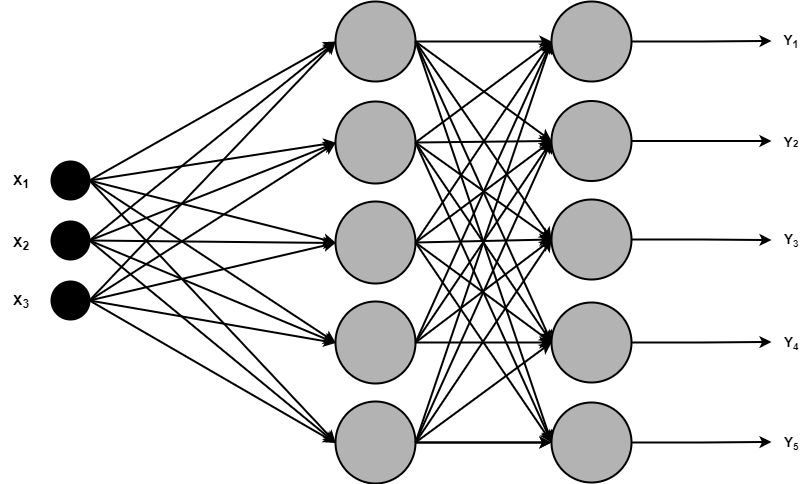
\includegraphics[scale=0.45]{figures/chapter3/FeedForward.png}
    \vspace*{5mm}
    \caption{Feed-Forward Network Structure}
    \label{fig:feed-forwardl}
\end{figure}

As seen in Figure \ref{fig:feed-forwardl}, each neuron in the first stage is connected to the neurons in the other layer. Combinations between all neurons require considerable high processing power which allow the solution of more complex problems. All neurons in the input layer direct their result to the output layer. If all the neurons between the layers are connected in a network, the network that is obtained can be called a fully connected network. On the other hand, if it is stated that the weight value between two different neurons, it is understood that there is no connection between that two neurons.

It is also pretty significant to state that single-layered perceptron models are only applicable to problems with linearly separable classes. Later on in the future, it is discovered that multi-layered perceptron networks can be used for non-linearly separable problems. Data distributions for different problems are given in figure \ref{fig:data-diff-dist}.

\begin{figure}[h!]
    \centering
    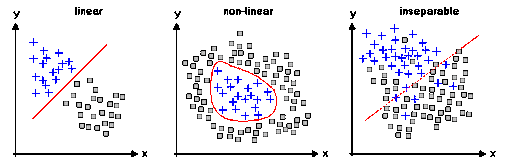
\includegraphics{figures/chapter3/linear-nonlinear-seperable.png}
    \caption{Data with Different Distributions\cite{sepdata}}
    \label{fig:data-diff-dist}
\end{figure}

Even though multi-layered perceptron networks are similar to single-layered perceptron networks, they contain fundamental differences. There are many more hidden layers in multi-layered perceptron. Also, another important difference is that the multi-layer perceptron has a backward stage in addition to the forward stage.

In forward stage, a path from the input layer to the output layer is followed. In oppose to that in the backward stage, an error is obtained from the value from the generated output and the value that should actually be obtained, and this error is used to change the parameters in the neurons which are weights and biases.

One other important addition is the usage of non-linear activation functions in multi-layer networks. With these improvements, multi-layered networks are able to work on non-linearly separable problems.

\subsection{Loss Function}

In mathematics, loss function also known as cost function is a function that represents the real “cost” of anyting to a real value. In essence, optimization problems try to minimize the output of the loss functions. They are designed to take one or more values as input and return a real number as output. Mean square error (MSE) is a simple loss function commonly used in neural network models. It is the sum of squared distances between the predicted values and the corresponding ground truth values. An optimizer will update the neural network parameterswhile trying to minimize this loss. Cross entropy loss \cite{cross_entropy}, also known as log loss or logistic loss, mostly used in classification problems when the values of the output layer is either zero or one. For binary classification problems binary cross-entropy loss can be used. If there are more than two classes in the problem categorical cross-entropy loss is preferred. In equation \ref{eq:binary_cross_entropy} the binary cross-entropy formulation is presented where \(y\) is the binary indicator if label is correct classified or not and \(p\) is the predicted probability of that label. To sum up, loss function is a mathematical way of measuring the error between the prediction and ground truth in order to see how the model is performing.

\begin{equation}
    L = -(y \cdot log(p) + (1-y) \cdot log(1 - p))
    \label{eq:binary_cross_entropy}
\end{equation}

\subsection{Optimizer}

Algorithms that try to minimize the output of the loss function by changing the model parameters during the training phase are called optimizers. Optimizers are algorithms that calculate how and how much should the values of parameters updated. One of the most popular optimizer used in neural network applications is the Gradient Descent algorithm \cite{gradient_descent}. Simply put, this algorithm looks at the gradient of the loss value effect of a small change in network parameters. In computer vision studies, advanced optimizers such as Adam \cite{adam} used.

\subsection{Activation Function}

Activation function is a spesific function for calculating the output of a single neuron in the neural network. Problems which are linearly non-seperable can be solvable using non-linear activation functions such as sigmoid, hyperbolic tangent (tanh), and ReLU. In concolutional layers ReLU activation function is commonly used. The main advantage of this activation function is that while casting negative neuron output values to zero it allows a regularization in the network via not activating every neuron. These mentioned activation functions can be seen in figure \ref{fig:activation_functions}.

\begin{figure}[h!]
    \centering
    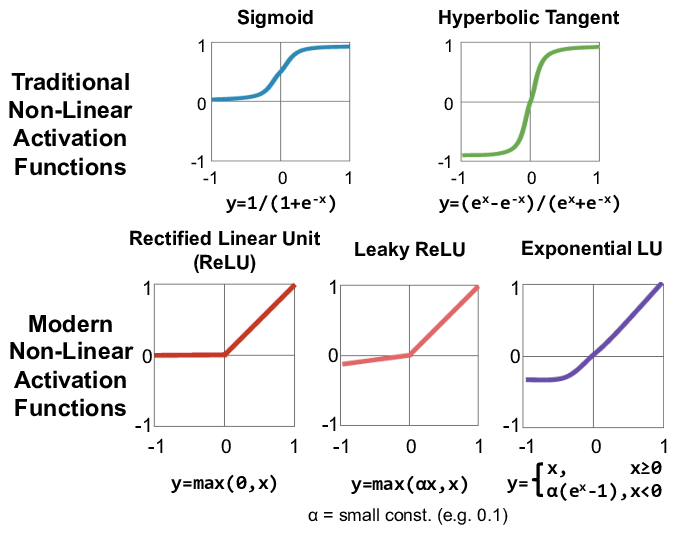
\includegraphics[width=10cm]{figures/chapter3/activation_functions.png}
    \caption{Activation Functions \cite{activation_functions}}
    \label{fig:activation_functions}
\end{figure}

\section{Convolutional Neural Networks}

Convolutional Neural Network is a widely used neural network architecture, especially thanks to its stunning success in computer vision studies \cite{leNet}. In this architecture, structures such as convolutional layer, pooling layer, flattening layer are used. CNNs are the structures that achieve only important features of the images by applying the convolution process using two-dimensional filters and obtaining different level of information in the image \cite{CNN_review}. CNN takes advantage of the hierarchical patterns in the data by following a path different than MLP structure. It brings together small and simple patterns to obtain more complex patterns. They use convolution operation in place of general matrix multiplication.

In the convolution layers, as seen in the figure \ref{fig:convolution}, 2D convolution is done between a tensor and the specified filter. In tasks such as inpainting where colored RGB images are used, these filters are applied separately to each color channel. During the convolution process while applying these filters which usually have 3x3, 5x5, or 7x7 size kernel onto matrix, on the borders padding process is applied. During this process, padding determines the course of action when values that are outside the limit and do not exist are desired to be accessed by convolution operation.

\begin{figure}[h!]
    \centering
    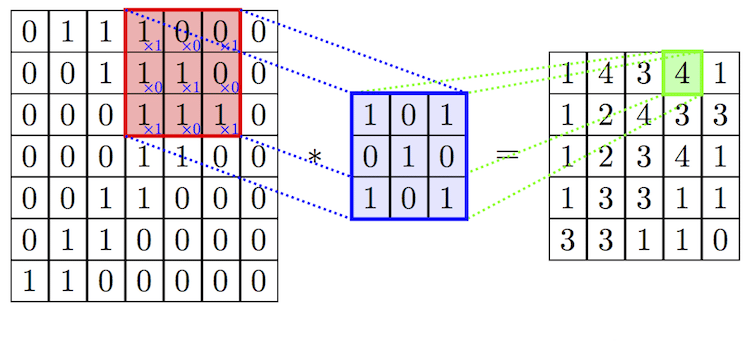
\includegraphics[width=10cm]{figures/chapter3/convolution.png}
    \caption{2D Convolution \cite{convolution_pooling}}
    \label{fig:convolution}
\end{figure}

Pooling layers, generally following the convolutional layers, reduce the size of the resulting tensor. In many convolutional neural networks, max pooling is used, but there are also min pooling and average pooling layers. The given tensor is divided into smaller pieces and a new and smaller tensor is obtained by taking the maximum, minimum or mean value of each sub-piece according to the chosen method. In figure \ref{fig:pooling}, average-pooling and max-pooling methods are shown.

\begin{figure}[h!]
    \centering
    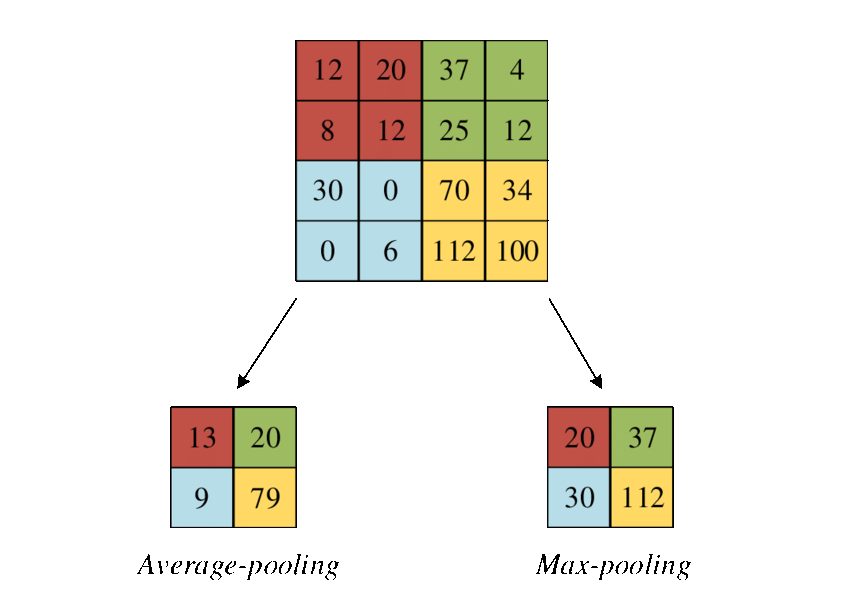
\includegraphics[width=10cm]{figures/chapter3/pooling.png}
    %\vspace{5cm} % gerekirse kullanabiliriz.
    \caption{Pooling \cite{convolution_pooling}}
    \label{fig:pooling}
\end{figure}

Flattening layer is the layer that makes the tensors in CNN structures vectorized in order to use the fully connected layers which commonly used in MLP structures. This layer serialized the incoming tensor and fills all the values to the neurons in layer.

There are two CNN architectures commonly used for deep inpainting studies. First one is the encoder-decoder structures, and the other one is a derivation of the former one which called as autoencoder structure. These architectures performs well on many computer vision task and also shows promising results on other inverse problems in computer vision such as inpainting, denoising, and super-resolution. Moreover, this structures can work on different deep learning problems such as sentiment analysis, image captioning, and translation. For example, Google Translate is built upon an encoder-decoder structure \cite{google_translate}.

\subsection{Encoder-Decoder Networks}

To explain briefly, encoder network can be in fully connected structure or convolutional structure or even as recurrent neural network (RNN) structure \cite{rnn_seq2seq}. An encoder network will take input and output a feature map which is simply a vector or more generally a tensor. This feature vector holds the necessary and important feature information about the input. The decoder network is usually the same network architecture as an encoder but in reverse. It takes a feature vector and tries to generate the input as closest as possible. Encoder-decoder network consist of two network parts which are an encoder and a decoder. Input processed through these structures. These network structures can be used in various areas such as language translation \cite{google_translate} and in computer vision applications as generative models. Mentioned model architecture can be seen in figure \ref{fig:encoder_decoder}.

\begin{figure}[h!]
    \centering
    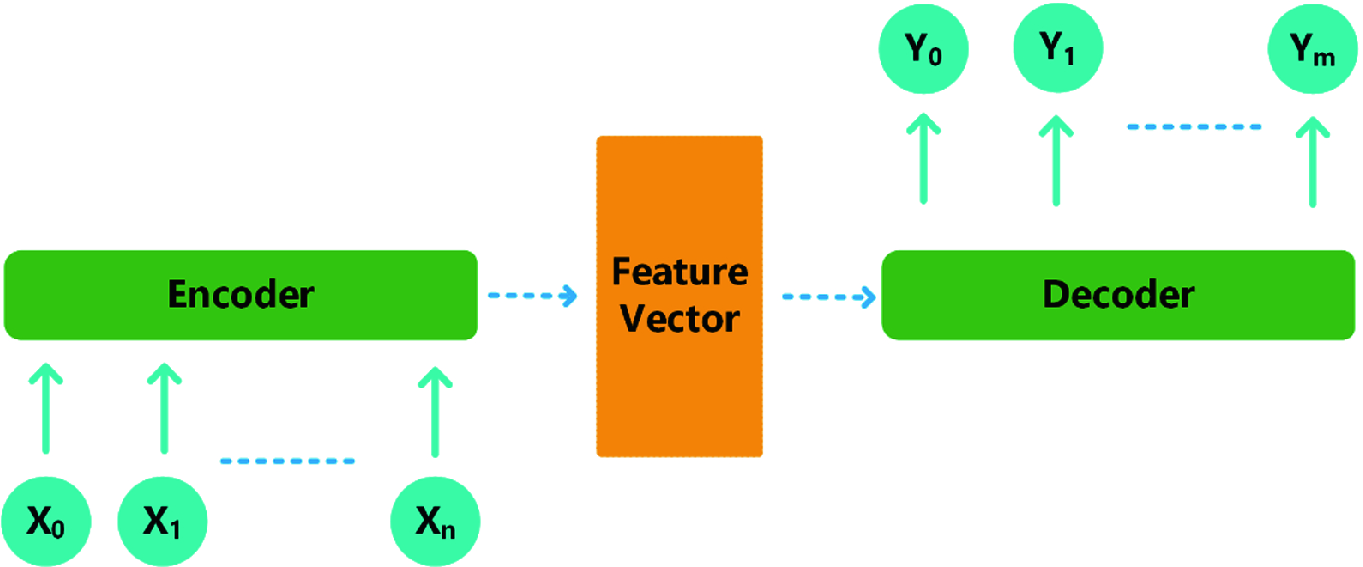
\includegraphics[width=10cm]{figures/chapter3/encoder-decoder.png}
    \vspace*{5mm}
    \caption{Encoder-Decoder Network Structure \cite{encoder_decoder}}
    \label{fig:encoder_decoder}
\end{figure}

\subsection{Autoencoder Networks}

Autoencoder is a structure that aims to establish a connection between input and output by obtaining a code in hidden layers. The code concept here can be considered similar to the feature vector in encoder-decoder network structures. The most typical use of autoencoders is dimension reduction. Autoencoder structured neural networks can be used in unsupervised non-linear dimension reduction applications. In figure \ref{fig:autoencoder_vs_pca} a comparison between a traditional dimension reduction method PCA \cite{pca} and a autoencoder structure.

\begin{figure}[h!]
    \centering
    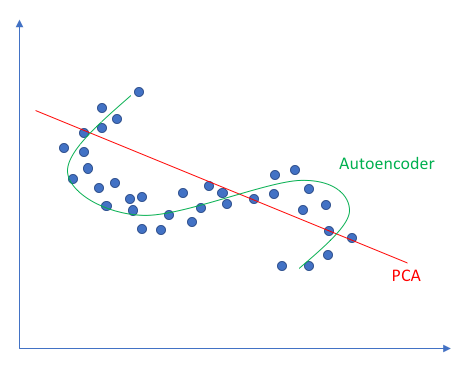
\includegraphics[width=9cm]{figures/chapter3/autoencoder_vs_pca.png}
    \caption{Autoencoder vs. PCA dimension reduction task \cite{autoencoder_vs_pca}}
    \label{fig:autoencoder_vs_pca}
\end{figure}

By training the autoencoders it becomes possible to ignore the noise in data. For instance, it can be used in anomaly detection application over any signal \cite{anomaly_detection1} \cite{anomaly_detection2}. Another example application would be to create a noiseless image from a noisy image by obtaining the most important features while ignoring the noise \cite{denoising}. This application is called denoising which is a popular inverse problems in computer vision studies. Learning with autoencoder structures is actually possible with an encoder that can best describe the input image and a decoder that can give an output as similar as possible to the original image using this description from former encoder structure. A convolutional autoencoder network structure designed for the image classification application is shown in the figure \ref{fig:mnist_autoencoder}.

\begin{figure}[h!]
    \centering
    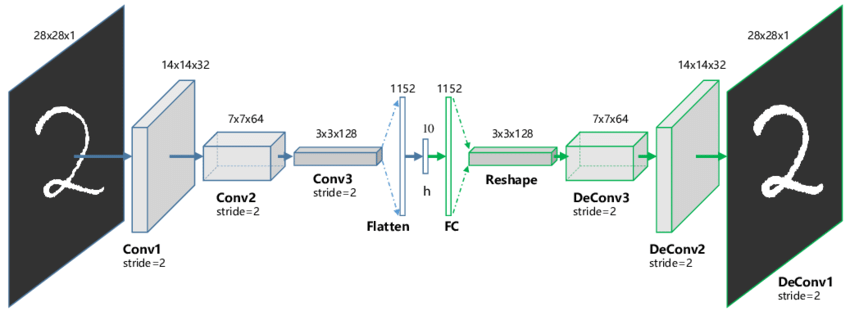
\includegraphics[width=13cm]{figures/chapter3/mnist_autoencoder.png}
    \vspace*{3mm}
    \caption{Convolutional autoencoder network structure \cite{autoencoders}}
    \label{fig:mnist_autoencoder}
\end{figure}

\section{Generative Adversarial Networks}

As time passed, many different machine learning methods and ideas emerged. As explained in the neural network and machine learning sections, these methods were methods that work to make operations on the input to obtain meaning, or methods that uses datasets with huge amount of data with expected outputs to converge the model to give correct result.

As machine learning methods and specifically neural network and deep learning methods began to be used more frequently and the number of areas in which they were used increased, the methods used continued to differ and develop. One of these ideas developed is Generative Adversarial Networks.

It is possible to categorize methods of machine learning under 2 main categories, which are supervised and unsupervised learning. Even, it is possible to obtain successful results with supervised learning labeling huge amount of data is not economical and highly time consuming or in some cases it is not possible. Basically, the basic idea behind the emergence of the generative models is that there is no possible data that can be compared with output, or rather, the desired output does not have a correct answer to compare. Objectives of generator and discriminator models is given in figure \ref{fig:gan1}.

\begin{figure}[h!]
    \centering
    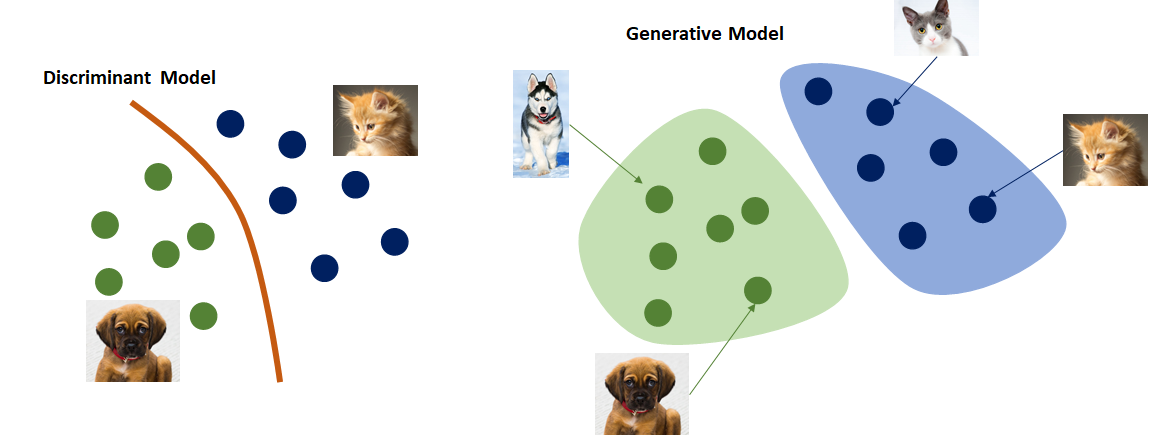
\includegraphics[scale=0.5]{figures/chapter3/generative-vs-discriminative-example.png}
    \vspace*{3mm}
    \caption{Difference Between Generative and Discriminative Models\cite{ganintro}}
    \label{fig:gan1}
\end{figure}

There are different type of generative methods in machine learning. Most generative models developed over Markov chain and maximum likelihood estimation. Also, there are generative models such as Restricted Boltzmann Machine \cite{Boltzman} and Deep Belief Network \cite{deepbelief}.  A new model called Generative Adversarial Networks (GANs) is proposed by Ian Goodfellow \cite{gan} and it has been used in various problems in the area of computer vision.

\begin{figure}[h!]
    \centering
    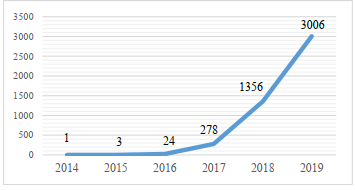
\includegraphics{figures/chapter3/gan-references-over-years.png}
    \vspace*{3mm}
    \caption{GAN Citation Counts \cite{ganoverview}}
    \label{fig:gancount}
\end{figure}

With the use and development of GANs in many different fields, GAN structures have become one of the leading methods of unsupervised learning. In figure \ref{fig:gancount}, work counts related to GAN is illustrated.

There are 2 different networks in the GAN. The word adversarial in its name comes from the fact that these structures work against each other throughout the training procedure.

As explained by Goodfellow \cite{gan}, within the GAN structure there are 2 networks being trained simultaneously. These networks are called generative and discriminative, respectively, G and D. In this structure, G is responsible for the creation of new data, while D tries to predict the probability of the data given as input to it.

From this point of view, it can be said that the Generative and Discriminator structures correspond to the minimax two-player game. Also, if G and D are constructed as perceptrons with multilayers, it can be said that the backpropagation can be used to train the whole structure. Simplified structure of GAN can be seen in figure \ref{fig:ganstruct}.

\begin{figure}[h!]
    \centering
    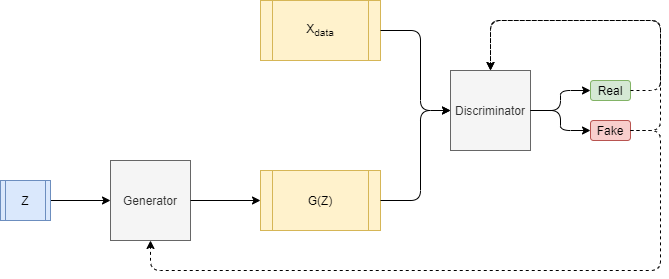
\includegraphics[scale=0.55]{figures/chapter3/GAN.png}
    \vspace*{3mm}
    \caption{GAN Model Explanation}
    \label{fig:ganstruct}
\end{figure}

When the mentioned adversarial model structure is implemented with perceptron, its application becomes straightforward. As a first step, generator structure G functions as a mapping to obtain data distribution from the input given to it. The discriminator structure created creates only a scalar as output. Structure D is trained to better label data from G and dataset. However, G is also trained to minimize log (1 - D (G (z))).

To explain, D and G play minimax with the function V (G, D) given in equation \ref{eqn:minmax}.

\begin{equation}
\label{eqn:minmax}
    min_Gmax_D V(D,G)= E_{x~P_{data(x)}}[logD(x)]+E_{z~P_{z}(Z)}[log(1-D(G(z)))]
\end{equation}

When implemented, it can be seen that Equation \ref{eqn:minmax} could not give sufficient results in the first steps of training. As can be guessed, at the beginning of the training phase, the Discriminator network could easily distinguish generated data from the real data which causes log(1-D(G(Z)) to saturate. In this case, it is reasonable to train to minimize log(D(G(Z)) rather than train to minimize log(1-D(G(Z)).

To exemplify the success of GAN structures, examples of faces produced by this method in different years are shown in Figure \ref{fig:gan-success}.

\begin{figure}[h!]
    \centering
    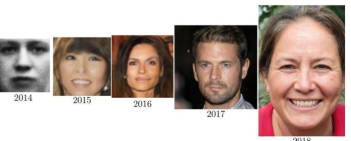
\includegraphics{figures/chapter3/gan-success-over-years.png}
    \vspace*{3mm}
    \caption{GAN Success Over Years \cite{ganoverview}}
    \label{fig:gan-success}
\end{figure}

\subsection{Deep Convolutional GAN}

Deep Convolutional Generative Adversarial Network \cite{dcgan}, shortly DCGAN, is a frequently used addition to GAN structures. The generator and discriminator used in this structure are in deep convolutional structure and thus a more stable training is performed. With this work, it is aimed to use the advantages of CNNs.

DCGAN is an important development in terms of having more successful and high quality generators. At the same time, this structure has helped the emergence of many different types of GAN structures. Overall structure of DCGAN is illustrated in figure \ref{fig:dcgan}.

\begin{figure}[h!]
    \centering
    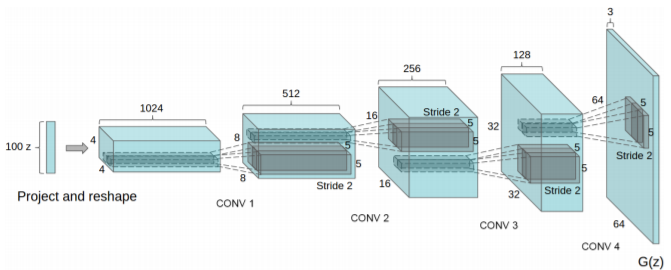
\includegraphics[scale=0.8]{figures/chapter3/dc-gan-structure.png}
    \caption{DCGAN Structure \cite{dcgan}}
    \label{fig:dcgan}
\end{figure}
\newpage
\subsection{Wasserstein GAN}

As GAN applications become widespread, different types of GAN structures have started to emerge. One of them is the Wasserstein GAN structure. This GAN structure both increases the stability of the GAN and provides the use of a loss function better related to the quality of the images produced.

WGAN model is a study presented by Arjovsky et al. \cite{wgan}, that adds additional features to the GAN structure. As mentioned earlier, images in the WGAN structure, receive a score that expresses the reality of the image rather than simply being classified as real or fake by the discriminator.

Fundamentally plans to be a solution to Discriminator and Generator balancing, one of the main problems of GAN structures, with the new Earth Move distance using WGAN. Earth-Mover distance is shown in equation \ref{eqn:wgan}.

\begin{equation}
\label{eqn:wgan}
    W(P_r, P_g)= {inf}_{y\epsilon\prod (P_r,P_g)}\mathbb{E}_{(x,y)~y}[||x-y||]
\end{equation}

\chapter{DEEP LEARNING METHODS}\label{deep_methods}

As with many different computer vision problems, deep learning methods have been used for image inpainting.
The reason why deep learning methods are being used more frequently as time progresses is that they provide more successful results in complex problems compared to traditional methods. The main reason for this is the creation of large-scale datasets that will enable the training of deep methods and the computational power that allow the training of these deep methods.

\section{CNN-based Methods}

Convolutional neural network structures, which are known to be very successful in computer vision studies thanks to their grid-like layer topology, are also used in image inpainting studies and give outstanding results. There are many architectures specially designed for inpainting work.

\begin{figure}[h]
    \centering
    \includegraphics{}
    \caption{U-Net Architecture}
    \label{fig:my_label}
\end{figure}

The U-Net [24] architecture used in Shift-Net inpainting [23] is one of them. This architecture takes an image and a mask which shows the missing areas and put them into convolutio layers. It concatenate the output of each layer with the corresponding layer of the same size in symmetrical architecture. The results of this structure achieve excellent success in terms of genereted image structure and fine detail.

\begin{figure}[h]
    \centering
    \includegraphics{}
    \caption{Shift-Net Architecture}
    \label{fig:my_label}
\end{figure}

Another popular architecture used in inpainting studies is the encoder-decoder network. Sidorov and Hardeberg [5] uses a 3D CNN encoder-decoder network architecture and can perform not only inpainting but also tasks such as denoising and super-resolution. In the study of Liu et al. [6] coherent semantic attention layer designed and used in an encoder-decoder structure called refinement network. This architecture can be seen in figure 6.

\begin{figure}[h]
    \centering
    \includegraphics{}
    \caption{CSA layer at the resolution of 32×32 in refinement network}
    \label{fig:my_label}
\end{figure}

In Artist-Net [7] proposed by Liao et al. In order to achive inpainting, two different content encoders, a style encoder used with a joint decoder. A similar structure is also available in CNN architecture developed by Cai et al. [1] for the purpose of semantic object removal. There are also context encoder [2] architectures used in inpainting studies. These context encoders basically CNNs trying to generate the missing parts of an image from their surroundings.

\begin{figure}[h]
    \centering
    \includegraphics{}
    \caption{Artist-Net Architecure}
    \label{fig:my_label}
\end{figure}

Zeng et al. [3] used Pyramid-context encoder network to perform inpainting. This pyramidal arthitecture called PEN-Net performs a high quality inpainting operation. The network structure can be seen in figure. Nakamura et al. [25] Aimed to remove the text from images and achieved excellent results using CNN.

\begin{figure}[h]
    \centering
    \includegraphics{}
    \caption{The Pyramid-context Encoder Network (PEN-Net)}
    \label{fig:my_label}
\end{figure}

\section{GAN-based Methods}

With different deep learning methods that have been tried over time, it has been analyzed that some methods give more successful results. It can be said that CNN and GAN based methods are better in evaluating realistic results in images. In this section, methods based on GAN idea will be explained. \newline
In the paper, Context Encoder: Feature Learning by Inpainting \cite{context_encoders}, it is shown that an encoder-decoder architecture, first create a feature space with its encoder. Then, the decoder uses that space the create realistic inpainted output image. Moreover, using different losses altogether shows significantly better and more realistic results could be constructed. Figure \ref{fig:context-encoder} illustrates the structure of Context Encoder.

\begin{figure}[h]
    \centering
    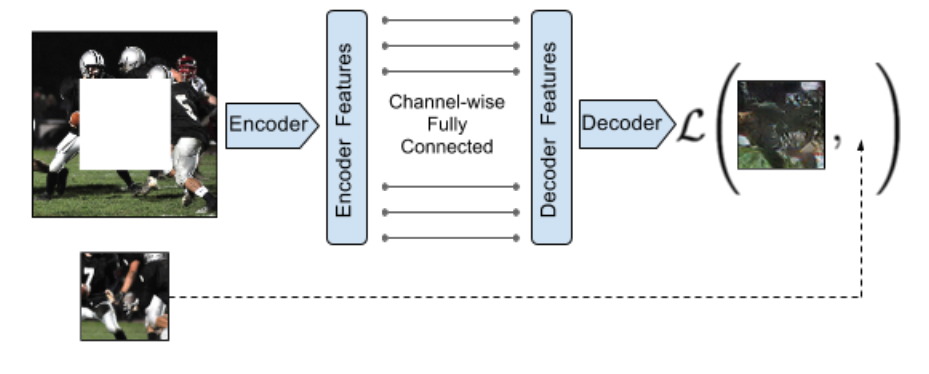
\includegraphics[scale=0.5]{figures/chapter4/context-encoder-example.png}
    \caption{Context Encoder Structure}
    \label{fig:context-encoder}
\end{figure}

In addition to this study, different methods have been proposed to solve different problems. To prevent blurry parts in the created pictures, using less downsampling layers are proposed by lizuka et al \cite{Iizuka2017}. Furthermore, using dilated convolution layers instead of fully connected layers are proposed by Yu and Koltun \cite{dilated_conv}. Unfortunately, these changes led to longer training times because of highly sparse filters generated by dilation element. Structure example with dilated convolution layers are presented in Figure \ref{fig:dilated-model}.

\begin{figure}[h]
    \centering
    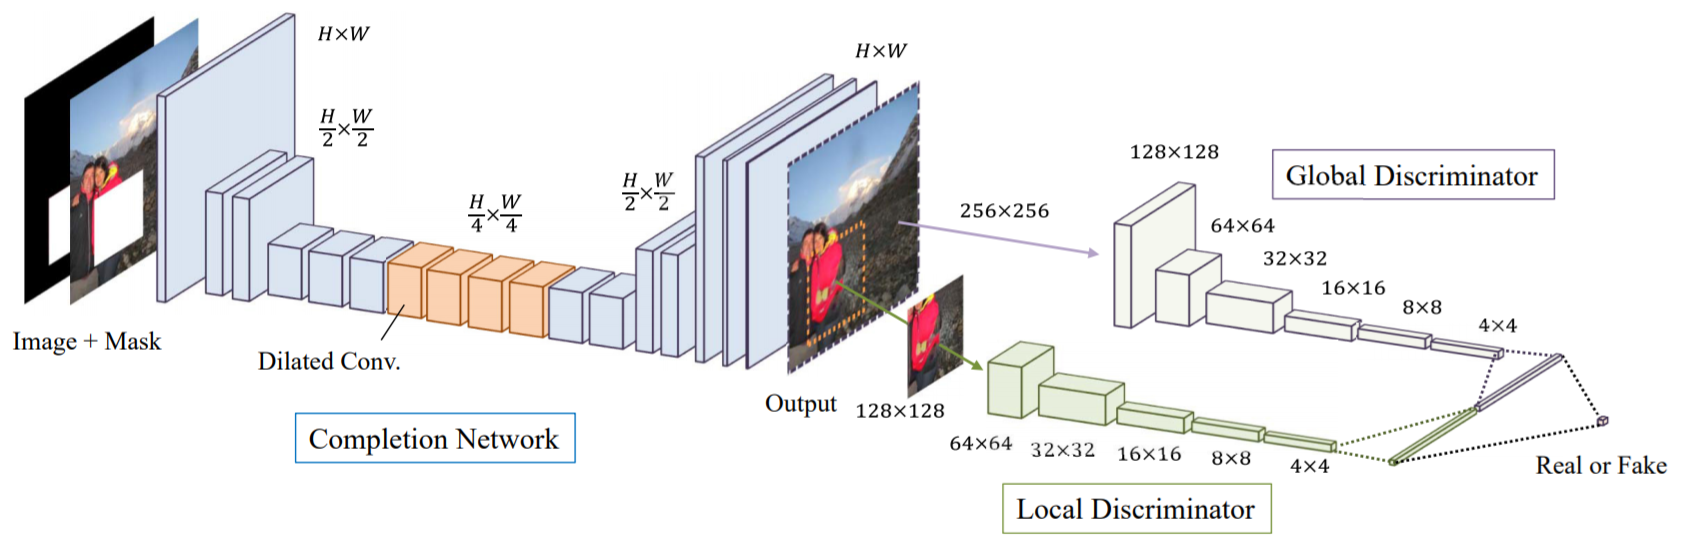
\includegraphics[scale=0.35]{figures/chapter4/Lizukaetal.PNG}
    \caption{Model with Dilated Convolution Layer}
    \label{fig:dilated-model}
\end{figure}

Different methods are also used such as using a pre-trained VGG network which leads to much shorter training time, proposed by Yang et al. \cite{inpainting_neuralpatch}. Also, Liu et. Al \cite{richer_conv_edge} came up with partial convolution layers that saves convolution filters from taking too many zeros from masked regions. Partial convolution operation is shown in Figure \ref{fig:partial-convl}.

\begin{figure}[h]
    \centering
    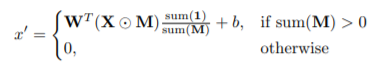
\includegraphics[scale=1]{figures/chapter4/partial-conv.png}
    \caption{Partial Convolution Operation}
    \label{fig:partial-convl}
\end{figure}

The novel idea that we actively use in our study and that provides the most successful results for the inpainting operation is the introduction of Generative Adversarial Networks asserted by Yeh et al \cite{semantic_inpainting_geneative}. Fundamental idea behind GAN is illustrated in Figure \ref{fig:gan-idedal} for an image related problem.

\begin{figure}[h]
    \centering
    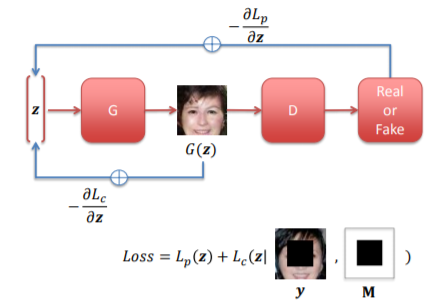
\includegraphics[scale=0.7]{figures/chapter4/GANinpainting.PNG}
    \caption{GAN Idea}
    \label{fig:gan-idedal}
\end{figure}

Different methods that use GAN structures and add many innovations to this structure will be explained in detail in the following sections.

\newpage
\section{State-of-the-Art Methods}

\subsection{EdgeConnect}

Nazeri et al. proposed a method \cite{edgeconnect} that uses edge information to produce realistic output images over missing zones.  EdgeConnect consists of 2 different GANs placed one behind the other. The first of these GANs tries to create the missing edge information over the masked image, and the second GAN structure complements the missing image by using this created edge information and the original masked image. Fundamental idea of the structure is shown in Figure \ref{fig:edgeconnect-network}.

\begin{figure}[h]
    \centering
    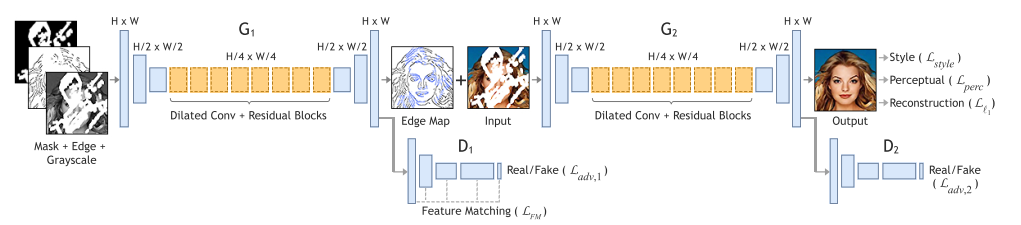
\includegraphics[scale=0.6]{figures/chapter4/EdgeConnect.PNG}
    \caption{EdgeConnect Network}
    \label{fig:edgeconnect-network}
\end{figure}

With this method, Yu et al want to solve some of the basic problems that arise in the inpainting process. Using the edge information, it is desired to create visuals with sharper borders. Figure \ref{fig:edgeconnect-example} demonstrates a few examples of inpainted images with EdgeConnect.

\begin{figure}[h]
    \centering
    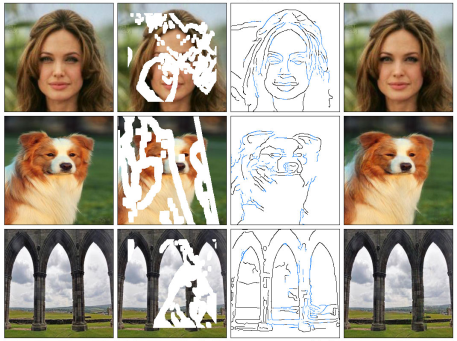
\includegraphics[scale=0.85]{figures/chapter4/ExampleEdgeConnect.PNG}
    \caption{EdgeConnect Inpainting Example}
    \label{fig:edgeconnect-example}
\end{figure}

Similar features are available for both structures that create edge information and final image. Generator Network consists of 3 parts. As mentioned before, an encoder structure is used primarily for feature extraction from the image. Residual network has been added after the encoder structure. Finally, there is a decoder to produce the image from features. Convolution layers are used adjacently for the discriminator structure.
The methods, transformations and tools we use to implement these structures will be explained in detail in the following sections.\newline
The working logic of the model basically consists of 4 steps. Briefly, the image selected as input in each iteration is directed to the dataset script. In this dataset script, the process of finding an edge and separating the image from the color channels are performed. From the parts obtained in this step, the edge and gray image are given to the edge model as input. The output is reverse masked and summed with the original parts. In this way, we only get the part produced about the masked region of the output picture. Then, with the edge information obtained from this section, the RGB image is given to the inpainted model and again reversely masked. \newline
Our goal was to implement the same model into our framework. To achieve this purpose, we got inspired by the example models that are publicly shared on internet. This was one of the main challenges on our project.  


\subsubsection{Edge Generator}

Edge generation is the fundamental idea behind EdgeConnect. In this section, generating edge will be explained.
Input image that is given to the system will be denoted as \(I_{gt}\), which stands for ground truth image. Also, edge information of input image and gray scale version of input image are denoted as \(C_{gt}\), \(I_{gray}\) respectively. Hence, while masked version of edge information and gray scale input images are represented as \(I^m_{gray}=I_{gray} \bigodot (1-M)\)  and \(C^m_{gt}=C_{gt}\bigodot(1-M)\), edge generation can be expressed as equation \ref{eqn:edge1}. In these operations, \(\bigodot\) represents Hadamard product.

\begin{equation}
\label{eqn:edge1}
    C_{pred} = G_{1}(I^{m}_{gray}, C^{m}_{gt}, M)
\end{equation}

\(C_{gt}\) and \(C_{pred}\) is given to discriminator network along with \(I_{gray}\), which tries to predict if the given edge map is real. In a greater scale whole network is trained using an objective function which is given in equation \ref{eqn:edge2} with adversarial loss and feature loss.

\begin{equation}
\label{eqn:edge2}
    min_{G_{1}}max_{G_{2}}\mathcal{L}_{G_{1}} = min_{G_{1}}(\lambda_{adv,1}max_{D_{1}}(\mathcal{L}_{adv,1})+\lambda_{FM} \mathcal{L}_{FM})
\end{equation}

In above equation, \(\lambda_{adv,1}\) and \(\lambda_{FM}\) are called regularization parameters and they are adversarial loss and feature matching loss respectively. Adversarial loss is given equation \ref{eqn:edge3}.

\begin{equation}
\label{eqn:edge3}
    \mathcal{L}_{adv,1} = \mathbb{E}_{(C_{gt},I_{gt})}[logD_{1}(C_{gt},I_{gray})]+\mathbb{E}_{I_{gray}}log[1-D_{1} (C_{pred}, I_{gray})]
\end{equation}

Feature-matching loss, pushes network to generate images more similar to real images from dataset which helps network to be more stable. Feature matching loss is given in equation \ref{eqn:edge4} below.

\begin{equation}
\label{eqn:edge4}
    \mathcal{L}_{FM} = \mathbb{E} [ \sum\limits^L_{i=1}{\frac{1}{N_i}|| D_1^(i) (C_{gt}-D_1^{i} (C_{pred})) ||_1} ]
\end{equation}

In given equation, \(N_i\) represents the number of elements in the activate layer numbered with i. \(D_1^{(i)} \) is discriminator’s activation in layer i and L is the discriminator’s last layer.

\subsubsection{Image Completion Network}

Inpainting network uses masked image which is expressed as  \(I^m_{gt}=I_{gt} \bigodot(1-M)\) to produce inpainted images over masked areas. Inpainting network also uses composite edge map which is defined as \(C_{comp}=C_{gt}  \bigodot (1-M)+C_{pred}  \bigodot M.\) Using these inputs, network produces an output with filled missing regions shown in equation \ref{eqn:edge5}.

\begin{equation}
\label{eqn:edge5}
    I_{pred} = G_2 (I^m_{gt}, C_{comp})
\end{equation}

Overall, image completion network is trained with joint losses which are \(\iota_1\) loss, adversarial loss, perceptual loss and style loss. Similar in edge generator adversarial loss is shown in equation \ref{eqn:edge6}. 

\begin{equation}
\label{eqn:edge6}
    \mathcal{L}_{adv,2} = \mathbb{E}_{(I_{gt},C_{comp})}[logD_{2}(I_{gt},C_{comp})]+\mathbb{E}_{C_{comp}}log[1-D_{2} (I_{pred}, C_{comp})]
\end{equation}

Other two losses that is used in image completion network is proposed in \cite{style} and \cite{perceptual} known as \(L_{perc}\)\space and \space \(L_{style}\).  Perceptual loss, penalizes the generated images if they are not similar perceptually to activation maps of a network that is trained before. Perceptual loss is shown in equation \ref{eqn:edge7}, where \(\phi_i\) is the activation map of pre-trained network on i’th layer.

\begin{equation}
\label{eqn:edge7}
    \mathcal{L}_{perc} = \mathbb{E}[ \sum\limits_{i=1}\frac{1}{N_i} || \phi_i(I_{gt}-\phi_i (I_{pred}) ) ||_1 ]
\end{equation}

Activation maps that are used in perceptual loss are also used in style loss which is expressed in equation \ref{eqn:edge8}.

\begin{equation}
\label{eqn:edge8}
    \mathcal{L}_{style} = \mathbb{E}_j [ || G_j^{\phi} (I^m_{pred})- G_j^{\phi} (I^m_{gt}) ||_1 ]
\end{equation}

\(G_j^\phi\) is Gram matrix that is obtained from previously shown activation matrix. Finally, overall loss function of the system is given in equation \ref{eqn:edge9}.

\begin{equation}
\label{eqn:edge9}
    \mathcal{L}_{G_2}=\lambda_{l_1}\mathcal{L}_{l_1} + \lambda_{adv,2}\mathcal{L}_{adv,2} + \lambda_{perc}\mathcal{L}_{perc} + \lambda_{s}\mathcal{L}_{style}
\end{equation}

\subsection{Generative Image Inpainting with Contextual Model}

One of the main problems in inpainting methods is that they create blurry and distorted parts in the missing regions. To prevent this, Yu et al. came up with Generative Image inpainting with Contextual Attention \cite{generative_contextual}.
Generative image inpainting with contextual attention consists of 2 main stages which are called Coarse Network and Refinement Network. Model structure is illustrated in figure \ref{fig:contextual-structure}.

\begin{figure}[h]
    \centering
    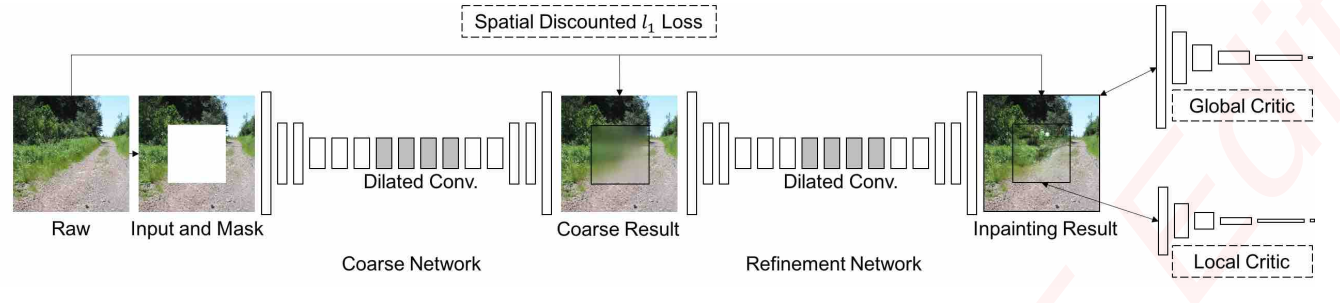
\includegraphics[scale=0.4]{figures/chapter4/GenerativeOverview.PNG}
    \caption{Contextual Attention Model Structure}
    \label{fig:contextual-structure}
\end{figure}

Coarse Network uses a method similar to the encoder and decoder structure like many methods previously described. In this part, an inpainted image is created over the missing part by using the GAN structure. \newline
The main idea of this study lies in Refinement network. The image created in this section progresses on 2 different paths, then the outputs of these 2 different paths are combined to achieve the desired improved result. Refinement network is shown in more detail in figure \ref{fig:refinement-network}.

\begin{figure}[h]
    \centering
    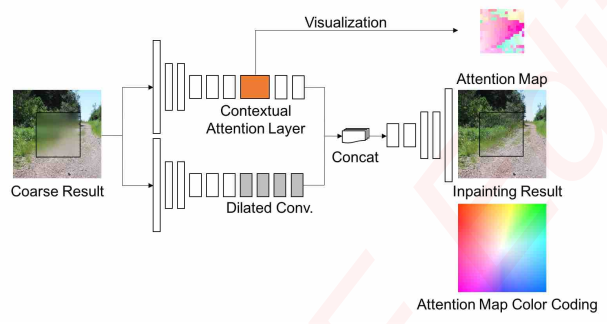
\includegraphics[scale=0.85]{figures/chapter4/GenerativeAttention.PNG}
    \caption{Refinement Network}
    \label{fig:refinement-network}
\end{figure}

In the first of these 2 paths, there is a structure consisting of dilated convolution and normal convolution layers. In the other and more important structure, there is a layer called Contextual Attention Layer that performs attention perception through the color map on the picture. In this layer, the picture is divided into patches and compared and evaluated. Algorithm in attention scoring is explained in Figure \ref{fig:attention-scoring}.

\begin{figure}[h]
    \centering
    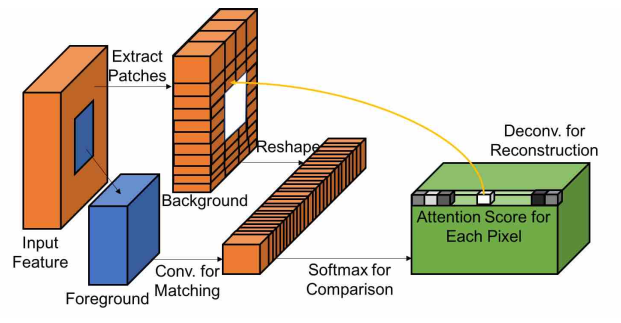
\includegraphics[scale=0.85]{figures/chapter4/GenerativeScoring.PNG}
    \caption{Refinement Network}
    \label{fig:attention-scoring}
\end{figure}

The Generative Contextual Attention Model has common similarities with the Edge connect model in terms of training. But there are critical differences due to the model type as expected. 

\subsubsection{Contextual Attention}

Contextual attention layer can fill the masked areas by using the feature information obtained from the unchanged parts of the image. For this, firstly, it divides the unmasked region expressed as background into patches and organizes it as a convolutional filter. Then it is put into the cosine similarity operation shown in equation [] with patches in the masked region expressed as foreground.

\begin{equation}
\label{eqn:context}
    s_{x,y,x^{'},y^{'}} = <\frac{f_{x,y}}{||f_{x,y}||}, \frac{b_{x^',y^'}}{||b_{x^{'},y^{'}}||}>
    % NEDEN HATA VERIYOR
\end{equation}

Where \(s_{x,y,x^{'},y^{'}}\) is patch similarity between background and foreground. Following this step, softmax function is used to obtain a similarity score with constant value \(\lambda\), as \(s^{*}_{x,y,x^{'},y^{'}} = softmax_{x^{'},y^{'} } ( \lambda_{s_{x,y,x^{'},y^{'} } } )\). In final step, used background patches are reused as deconvolutional filters to reconstruct foregrounds. For better results, attention coherency could be increased by calculating a new attention score by summing scores in a shifted direction in desired axis.

\subsection{Image Inpainting via Generative Multi-column CNN}

In the article [ref:gmcnn], the inpainting process is presented with a multi column CNN structure. This network acquires different image features in parallel. A new reconstructon loss function has been developed to better characterize global objects. Also, a loss function called ID-MRF loss has been developed to increase the local details and improve the texture quality. With these loss functions and a adversarial loss, the model trained on the image dataset can fill the masked pixels in an image with local and global information. Trained model of this architecture shows realistic results without even the need for post-processing, which is often seen on similar works.

This inpainting system has a structure that can be trained from begining to end. It first receives an image and a binary mask as input. The pixels to be masked are denoted by 1 and known pixels by 0. Then the image masked by the  operation and inserted into the network. The result of the network is a completed image. Network structure is as shown in the figure 3.5.1.

\begin{figure}[h]
    \centering
    \includegraphics{}
    \caption{Network structure of the GMCNN}
    \label{fig:my_label}
\end{figure}

The network structure shown in figure 3.5.1 consists of three sub-networks. The first one is the generator network that creates the output painted image and is the main network which will used after the training phase.The other two sub-networks are networks that are only needed during the training phase respectively, local and global discriminator networks which used to calculate the adversarial loss and a pre-trained VGG network [ref:simonyan] in order to calculate the designed ID-MRF loss. Generator network consists of n parallel encoder-decoder branches (in figure 3.5.1, n = 3). These structures consist of convolution layers that apply filters of different kernel sizes to the input tensor. These convolution layers obtain features at different frequency levels according to the kernel size. Next, these branches which have different levels of information about input image upsampled bilinearly to the original image size. Then these same size branches combined together and forms a feature map. Continued with two more convolution layers, this feature map is transformed into the image. This image is the generated output image of the network and it is used to calculate the network loss when compared to the ground truth image. Even though these branches seem to be independent from each other, they are actually affected by the backpropagation phase in the training process. This framework is different from the commonly used encoder-decoder structures. In an encoder-decoder network, every layer inherits its information from its previous layer. However, in this architecture, different structures complement each other instead of just inheriting. With these different representation levels, the inpainting process is carried out.

To calculate loss during model training, a mixture of three loss functions used. ID-MRF loss, reconstruction loss, and adversarial loss.

ID-MRF stands for implicit diversified Markov random fields. This loss function is used to train with a path similarity based approach within a VGG structure fed with generated results. This method, which is used only during the training phase, is a metric used to measure the similarity between the randomly selected patches between generated pixel areas and the ground truth area pixel areas. A simple similarity measure like cosine similarity can be used to compute this process. This metric measures the similarity between the generated content and the random selected nearest-neighbor patches. But using cosine similarity measurement has some limitations. As seen in the figure 3.5.2.a, the results often become like blurry textures and for large masking areas this can become a serious problem.

\begin{figure}[h]
    \centering
    \includegraphics{}
    \caption{Cosine similarity vs. Relative similarity}
    \label{fig:my_label}
\end{figure}

In this article, in order to eliminate this problem, a relative similarity measurement has been developed and used instead of a direct similarity such as cosine similarity. As seen in figures 3.5.2.b and 3.5.2.c, the ground truth image pathches compared with the generated image patches. This relative similarity [ref: rmerc] equation can be seen in figure 3.5.3.

\begin{equation}
    buraya equation gelecek
\end{equation}

u(v, s) in the equation represents cosine similarity between patch v from generated area and patch s from ground truth area, the  and  values are constants, and  represents the features on the Lth layer of the pre-trained VGG network. To be more precise, let generated content denoted as  and  is the corresponding ground truth, for any layer L, ID-RMF loss can be calculated as equation in the figure 3.5.4.

\begin{equation}
    buraya equation gelecek
\end{equation}

The  is the normalized relative similarity as in the figure 3.5.5 and Z is normalization factor. r and s represents the patches from generated image and ground truth image respectively.

\begin{equation}
    buraya equation gelecek
\end{equation}

If all r patches in the  are close to only one spesific patch and far from other patches in ground truth, relative similarity becomes small and leads to a big loss value (L). On the other hand if every r patch from generated image has a similar corresponding s patch in ground truth image, relative similarity becomes big and leads to a small loss value. One of the biggest contributions of this measure is to increase the similarity between the  and  features. While minimizing the loss, generated feature distrubution and ground truth feature distrubution approach each other. As a result, in the inpainting regions blurry texture problem is overcome and variation is achieved.

\begin{equation}
    buraya equation gelecek
\end{equation}

With this loss active, during the training phase, a realistic texture was obtained both locally and globally. The features layers mentioned and shown in the figure 3.5.6 are taken from the VGG19 pre-trained model [ref:vgg].

A pixel-wise working reconstruction loss has been developed as a spacial variant reconstruction loss. In this designed confidence-driven reconstruction loss, known pixel values assigned with the value of 1 and others missing pixels confidence values gradually decays with respect to the distance from the mask border. Thus the pixels on the boundary make the most impact on the loss. As a result, a smooth transition between the masked area and the rest of the image is achieved. Increasing distance away from the boundary is obtained by convolving the mask with a gaussian filter and formulized like equation in the figure 3.5.7.

\begin{equation}
    buraya equation gelecek
\end{equation}

g represents a 64×64 gaussian filter with standart deviation of 40 and ◎ is the Hadamard product operator. Loss weight mask  is obtained by repeating the equation in figure 3.5.7 several times. Lastly the reconstruction loss calculated with the formula in the figure 3.5.8.

\begin{equation}
    buraya equation gelecek
\end{equation}

In figure 3.5.8, G([X,M];θ) represents the generated output. With the help of this loss, the results are softened from the mask boundaries towards the center.

Adversarial loss is used frequently in many tasks such as inpainting missing pixels. In this architecture, improved Wasserstein GAN [ref:gulrajani] is used as a generator and one local and one global structure are used together as a discriminator. Reason for using two discriminators is to overcome the problem when generated areas are realistic and low loss but ill-matched with the rest of the image. The adversarial loss function is defined as in figure 3.5.9, where X = tG([X, M]; θ) + (1 − t)Y and t  [0, 1].

\begin{equation}
    buraya equation gelecek
\end{equation}

Finally, the three loss functions mentioned above are combined together with different weights denoted as  and . Regularization of the model achieved in training process.

\begin{equation}
    buraya equation gelecek
\end{equation}

As a comparison with GMCNN, two other CNN-based inpainting architectures selected under same conditions with the same losses and same hyperparameters. A single encoder-decoder network and the previously mentioned contextual attention coarse network [ref:context] tested alongside with the GMCNN. Results are shown in figure 3.5.11.

\begin{figure}[h]
    \centering
    \includegraphics{}
    \caption{GMCNN Comparison}
    \label{fig:my_label}
\end{figure}

Also our implementation of the GMCNN using a pretrained network, achieved great results with two different datasets. Places [ref] dataset model and CelebA [ref] dataset model outputs can be seen in the figures 3.5.12 and 3.5.13 respectively.

\begin{figure}[h]
    \centering
    \includegraphics{}
    \caption{Result of the model trained on Places2 dataset}
    \label{fig:my_label}
\end{figure}

As a limitation, like most of the generative neural networks this network also struggle with large datasets with diverse classes such as ImageNet. It is a harsh challange to inpaint different objects and places with one pre-trained model.

\begin{figure}[h]
    \centering
    \includegraphics{}
    \caption{Result of the model trained on CelebAHQ dataset}
    \label{fig:my_label}
\end{figure}

\subsection{Deep Image Prior}

Deep convolutional networks have become very popular for image generation and restoration problems. In general, the reason behind the good results of such networks is the ability to obtain realistic image priors from datasets containing large number of images. To explain briefly what image prior is, it is a general definiton for the information on an image that can be used for any kind of image processing tasks to enhance results, to choose the processing parameters, and resolve indeterminacies. For instance, some information about an image may known such as color distrubution, and this information or its approximation can be used as a prior to a spesific task. Image priors can be represented with math form and merged into processing steps such as filtering, deconvolution and segmentation which helps to reduce the feasible solutions.

In the article [ref: deepimageprior], the authors show that a generator network structure can get enough low-level image statistics without a long training phase on any dataset. To prove this hypothesis, designed deep image prior method with a randomly-initialized convolutional neural network was used as a prior and highly competitive results were obtained in various inverse computer vision problems such as denoising, super-resolution, and image inpainting. What makes this method important except that it can be used in a wide range of cumputer vision research areas, it can also forms a new branch between learning-based networks and learning-free networks with fixed explicit priors like self-similarity etc. To be declared in a single sentence, in deep image prior, authors tries to bridge the gap between two popular methods by constructing a new explicit prior using convolution neural network.

To perform the task of image restoration like inpainting, learned-prior and explicit-prior are the two common methods utilized by researchers. To explain with an example, learned-prior is a straight forward approach to train a deep convolution network to learn about the world through the dataset. On the other hand, explicit-prior or hand-crafted prior method, is embedding constrains and distinctly teaching what types of images are natural. However in real word it is extremely difficult to express constraints mathematically. As a result, most of the explicit-prior methods works poorly compared to a state-of-the-art pre-trained neural network, yet deep image prior method offers surprisingly good results which can compete with learned-prior methods.

Deep convolutional networks are architectures that on of the best for solving inverse image problems. Architectures like generative adversarial networks and variational auto-encoders achieve state-of-the-art solutions on this tasks. However, it is not entirely correct to assume that the reason for the amazing results of these models trained on large datasets is that they can capture realistic image priors while learning over the data. Because only a good learning curve on a selected datasets does not prove that a network performs good on an image from a different dataset. A good network requires generalization which means that the structure of the network should resonate with the structure of the given input data. For example, as shown [1], an image classification network which successfully generalized for real data can overfit when a random labels are presented.

To put it more clearly, in this article the authors shows that learning process is not a requirement and it is possible to obtain quite good image priors with a convolutional generative structure that does not need training. In order to prove this claim, an untrained, randomly-initialized convolutional generator neural network is fitted on a given corrupted image. Generator network initialized with a random distrubution conditioned to the input corrupted image. The reconstruction task is expressed as a conditional image generation problem. Randomly initialized network weights optimized without needing any other data than input image and network itself. “Only prior information is in the structure of the network itself.” [] as authors states.

\begin{equation}
    buraya equation gelecek
\end{equation}

In figure 3.6.1, x is corrupted input image, z is a code tensor and  represents the network parameters which randomly initialized in the beginning and will map code tensor z to the image x while resolving inverse problem through iterations. The network is switching between filtering operations such as non-linear activation, convolution, and upsampling. For most of the experiments, a hourglass type U-Net architecture with two million parameters used.

In image restoration problems the goal is to recover original image x, when having a corrupted image. To solve such tasks, problem is often formulated as an optimization like in figure 3.6.2.

\begin{equation}
    buraya equation gelecek
\end{equation}

In equation 3.6.2, E(x;) is a data term dependent to the task and R(x) is an image prior. For a wide range of problems, such as super-resolution, denoising, and inpainting, the data term is typically simple to design, while designing the image prior is a challenging. For inpainting problems, the corresponding data term is defined as in the equation 3.6.3.

\begin{equation}
    buraya equation gelecek
\end{equation}

The symbol ◎ is the Hadamard product operator and m is the binary mask applied onto ground truth image x. The goal is to reconstruct the ground truth image x from the given image  with missing pixel values.

As mentioned, choosing a regularizer R(x) that can catch general priors in image x is a difficult and very extensive research subject within itself. To give an example, if total variation (TV) is selected as a regularizer, the results are often have uniform regions [ref: mahendran]. In this study, as seen in the equation 3.6.4, implicit prior which gathered from neural network was used as a regularizer.

\begin{equation}
    buraya equation gelecek
\end{equation}

* is the minimizer achieved with the help of the gradient descent optimizer from random parameter values. Result of the inpainting process denoted as x* is given in figure 3.6.4. It is also possible to apply minimazation on the code tensor z. However here z is a fixed three dimensional tensor containing 32 feature maps of uniform noise with the same spatial size as x.

\begin{figure}[h]
    \centering
    \includegraphics{}
    \caption{Deep Image Prior Comparison}
    \label{fig:my_label}
\end{figure}

In the figure 3.6.5, deep image prior method compared with Shepard Neural Networks [ref:shepard] which is particularly designed for inpainting applications. Using a black text as a mask, this method demonstrates astonishing results. While in the output of the Shepard network remainings of the mask can be seen, in the output of the deep image prior method there are almost no artifacts.

\begin{figure}[h]
    \centering
    \includegraphics{}
    \caption{Deep Image Prior output}
    \label{fig:my_label}
\end{figure}

In another experiment, deep image prior is compared with Convolutional Dictionary Learning method [ref: dictionary] using an image where as a mask half of the pixels are removed by applying a bernoulli distrubution with random noise. Visual comparison is given in figure 3.6.6.

Apart from the inpainting study of small pixel regions, a large region inpainting process was also tested and deep image prior method has shown great success again. Although deep image prior method works great for variety of images, as a limitation it works poorly while inpainting large masked areas of the images which have highly semantic information such as face images due to being a learning-free method.

\begin{figure}[h]
    \centering
    \includegraphics{}
    \caption{Deep Image Prior output}
    \label{fig:my_label}
\end{figure}

Result of the inpainting of a large masked region with deep image prior method is compared with a learning-based generative adversarial network model [ref: global-local]. As shown in the figure 3.6.7, the pretrained GAN structure performs the inpainting process with the information learned from the dataset it trained on. On the other hand deep image prior fills the missing region with texture information learned from known regions.

As mentioned, deep image prior is a method which can be applied onto any network architecture, the results obtained are highly dependent on the network structure used. In figure 3.6.7, deep image prior method applied on different neural networks. From the results, it can be concluded that deeper networks have positive effect on the inpainting solution. However, having skip-connections which can significantly improve image recognition tasks shows extremely harmful behaviour in inpainting process as seen in figure 3.6.8.e and 3.6.8.f where skip-connectons added to the ResNet [ref] and U-Net [ref] architectures.

\begin{figure}[h]
    \centering
    \includegraphics{}
    \caption{Skip Layer effects}
    \label{fig:my_label}
\end{figure}

Finally, we tested the Deep Image Prior method using a encoder-decoder network and achieved quite enough results. Figure 3.6.9 shows the output after 1000 iteration.

\begin{figure}[h]
    \centering
    \includegraphics{}
    \caption{Result of the 1000th iteration of an encoder-decoder network}
    \label{fig:my_label}
\end{figure}
\chapter{EVALUATION, RESULTS AND OUR CONTRIBUTION }\label{our_work}

The most important part of our study is to implement these models we have examined and to make comparisons of these models after the implementation. While implementing these models, we basically used the python software language, but we also used many different libraries and frameworks. The main 2 libraries we used are pytorch and tensorflow. However, we also used libraries like matplotlib, openCV, and numpy. The structures and codes we use can be accessed on the internet in an open source manner.
\newline
Implementing Deep Learning models is always a challenge. For this purpose, we used frameworks that allow us to use graphic cards for training and test phases. Similar to all studies on inpainting we used places2 dataset \cite{dataset_places} for training and test. However due to high computational power and relatively weak GPUs we had, we needed to decrase the size of the dataset we used. An example batch from places2 dataset is shown in figure \ref{fig:dataset}

\begin{figure}[h!]
    \centering
    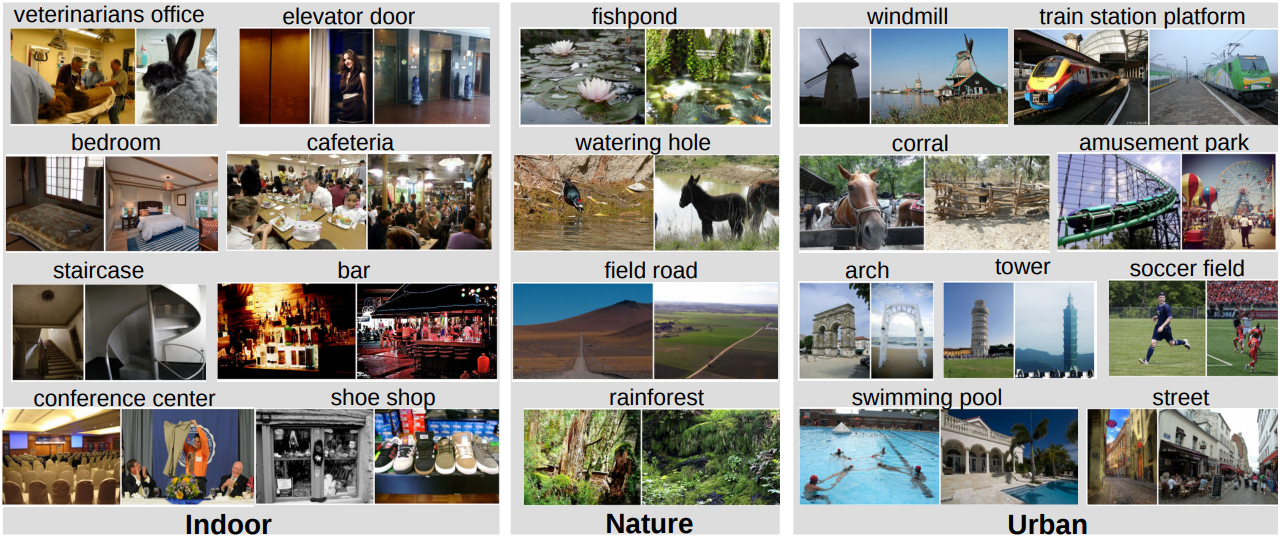
\includegraphics[scale=0.45]{figures/chapter5/Places2Dataset.PNG}
    \vspace*{4mm}
    \caption{Places2 Dataset \cite{dataset_places}}
    \label{fig:dataset}
\end{figure}

Example visual results and mathematical results over a validation dataset for different types of masks are represented in the following sections.  
\newpage
\section{Framework}

One of the key points in our study was to create a model that allows many different models to work together. In order to achieve this, we had to create a framework that is easily accessible by different models and consists of parts that generate standard types of feedback. In this way, we would have obtained a modular structure where it is easy to make changes and incorporate new ideas. General structure of our framework is shown in Figure \ref{fig:framework}.

\begin{figure}[h!]
    \centering
    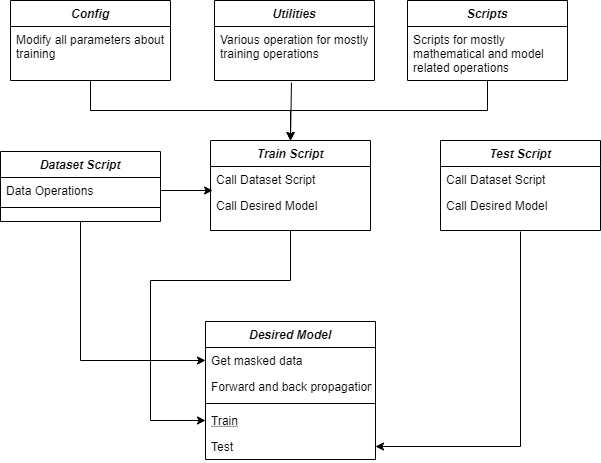
\includegraphics[scale=0.55]{figures/chapter5/framework (1).png}
    \vspace*{4mm}
    \caption{Framework}
    \label{fig:framework}
\end{figure}
In order to provide these, we created scripts that will serve as small building blocks. The most important of these building blocks are the dataset and utilities scripts, which are also actively used by models and can include important features of the models.
\newline
Masked images or transformed images that models use as input are also generated by the dataset script. We created 2 different types of masking. The first masking type we have created is the masking type that creates scattered lines on the picture which we call line masking. With this masking type, we are able to simulate smaller imperfections rather than large missing regions in the picture. Line masking example is shown in figure \ref{fig:linemasking}.

\begin{figure}[!ht]
    \centering
        \subfloat[Image]{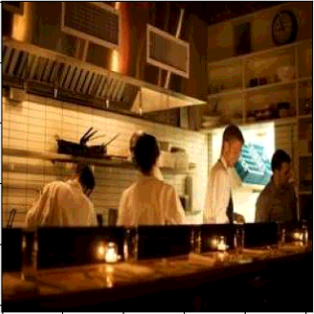
\includegraphics[width=0.3\columnwidth]{figures/chapter5/maskingtypes/line1.PNG}}
        \hspace{0.02\columnwidth}
        \subfloat[Mask]{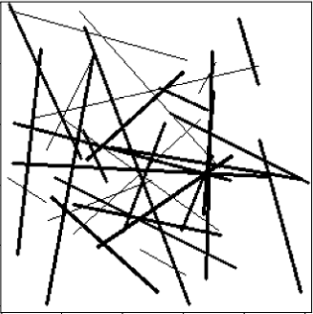
\includegraphics[width=0.3\columnwidth]{figures/chapter5/maskingtypes/line2.PNG}}
        \hspace{0.02\columnwidth}
        \subfloat[Masked Image]{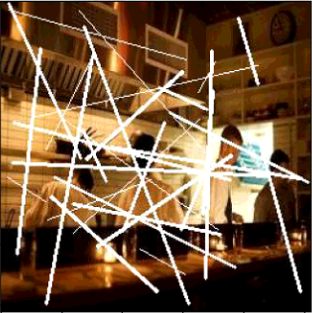
\includegraphics[width=0.3\columnwidth]{figures/chapter5/maskingtypes/line3.PNG}}
    \vspace*{3mm}
    \caption{Line Masking Example}
    \label{fig:linemasking}
\end{figure}

The other masking function we use is a function that masks a region of the given ratio value, starting from a random point on the picture. We preferred to use this masking type more to show that generative models are more successful. Our second masking type is presented in figure \ref{fig:percentagemasing}.

\begin{figure}[!ht] 
    \centering
        \subfloat[Image]{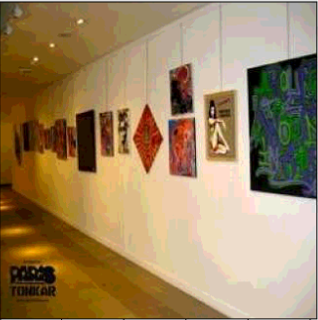
\includegraphics[width=0.3\columnwidth]{figures/chapter5/maskingtypes/percentage1.PNG}}
        \hspace{0.02\columnwidth}
        \subfloat[Mask]{
\includegraphics[width=0.3\columnwidth]{figures/chapter5/maskingtypes/percentage2.PNG}}
        \hspace{0.02\columnwidth}
        \subfloat[Masked Image]{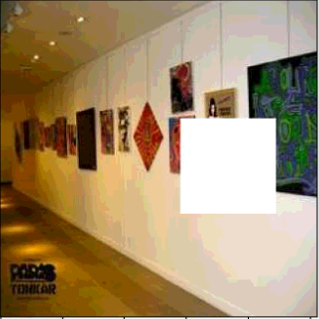
\includegraphics[width=0.3\columnwidth]{figures/chapter5/maskingtypes/percentage3.PNG}}
    \vspace*{3mm}
    \caption{Percentage Masking Example}
    \label{fig:percentagemasing}
\end{figure}

Image inpainting, unfortunately, is not a method whose success can be fully controlled with mathematical criterias. However, PSNR and SSIM values will be used throughout the project as a criterion in addition to achieving personal realistic results. Also for out comparisons mathmatical methods are used throughout our project. An example of image inpainting with one of our mathematical method which uses navier-strokes method is shown in Figure \ref{fig:mathmodel}.

\begin{figure}[!ht]
    \centering
        \subfloat[Input Image]{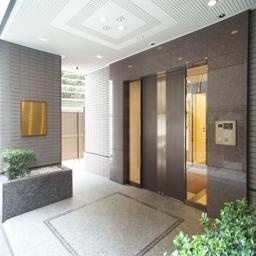
\includegraphics[width=0.3\columnwidth]{figures/chapter5/fpnvsvanilla/data1.jpg}}
        \hspace{0.02\columnwidth}
        \subfloat[Mask]{
\includegraphics[width=0.3\columnwidth]{figures/chapter5/fpnvsvanilla/data1mask.png}}
        \hspace{0.02\columnwidth}
        \subfloat[Navier-Strokes Output]{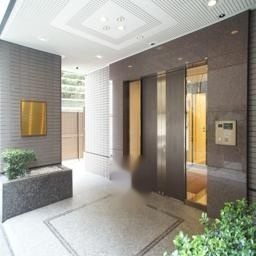
\includegraphics[width=0.3\columnwidth]{figures/chapter5/mathmodel/mathdata1.png}}
        \hspace{0.02\columnwidth}
        \subfloat[Input Image]{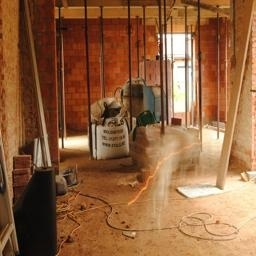
\includegraphics[width=0.3\columnwidth]{figures/chapter5/fpnvsvanilla/data2.jpg}}
        \hspace{0.02\columnwidth}
        \subfloat[Mask]{
\includegraphics[width=0.3\columnwidth]{figures/chapter5/fpnvsvanilla/data2mask.png}}
        \hspace{0.02\columnwidth}
        \subfloat[Navier-Strokes Output]{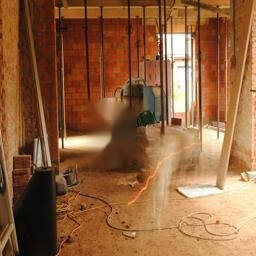
\includegraphics[width=0.3\columnwidth]{figures/chapter5/mathmodel/mathdata2.png}}
        \vspace*{3mm}
        \caption{Mathematical Model Example}
    \label{fig:mathmodel}
\end{figure}

\section{Our Contribution}

In addition to the examined methods, two new methods are proposed and implemented in our project called, Unified Contextual-Edge Model and FPN GAN Model.

\subsection{Unified Contextual-Edge Model}
During our literature review we studied a model by Yu et al. which is called Free-Form Image Inpainting with Gated Convolution \cite{freeform_inpainting}. In this model, there are 3 main stages as shown in the Figure \ref{fig:freeform}.

\begin{figure}[h!]
    \centering
    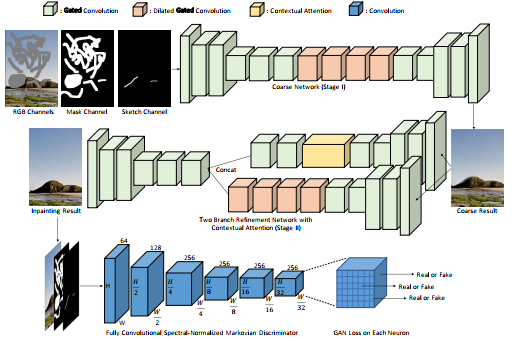
\includegraphics[scale=0.7]{figures/chapter5/Free-form.PNG}
    \vspace*{3mm}
    \caption{Free-form Image Inpainting Example \cite{freeform_inpainting}}
    \label{fig:freeform}
\end{figure}

Based on this, we wanted to try EdgeConnect and Generative Contextual Attention models in a cascaded network. Hence, there will be 3 steps in the new model. Which consists of following steps. figure \ref{fig:unifiedIdeda} shows the steps of this model. 


\begin{figure}[h!]
    \centering
    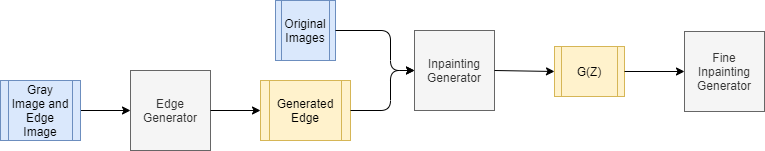
\includegraphics[scale=0.5]{figures/chapter5/Unified.png}
    \vspace*{3mm}
    \caption{Unified Model Structure }
    \label{fig:unifiedIdeda}
\end{figure}

•	Edge information prediction \newline
•	Inpainting operation with edge and RGB image as input \newline
•	Refinement network  \newline
We were able to implement this idea. However, size of the model is nearly doubled and training time is significantly increased, but it was also possible to use independently trained parameters for our models. Figure \ref{fig:unifiedexample} shows the obtained result with unified model.

\begin{figure}[!ht]
    \centering
        \subfloat[Input Image]{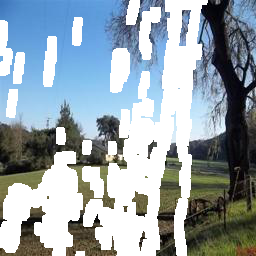
\includegraphics[width=0.45\columnwidth]{figures/chapter5/inputs/places2_05.png}}
        \hspace{0.05\columnwidth}
        \subfloat[Inpainted Image]{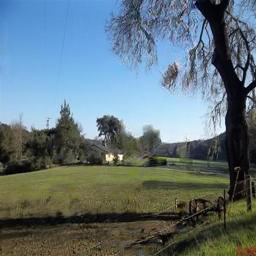
\includegraphics[width=0.45\columnwidth]{figures/chapter5/UnifiedOutput/places2_05.png}}
        \hspace{0.05\columnwidth}
        \subfloat[Input Image]{\includegraphics[width=0.45\columnwidth]{figures/chapter5/inputs/places2_06.png}}
        \hspace{0.05\columnwidth}
        \subfloat[Inpainted Image]{\includegraphics[width=0.45\columnwidth]{figures/chapter5/UnifiedOutput/places2_06.png}}
        \vspace*{3mm}
        \caption{Unified Model Inpainting Example}
    \label{fig:unifiedexample}
\end{figure}

\subsection{Feature Pyramid GAN Model}
Feature Pyramid Networks is proposed in paper Feature Pyramid Networks for Object Detection \cite{feature_pyramid}. FPN is commonly used in object detection problem. The basic idea behind FPN is to combine the feature information of different sizes of the same image to obtain a more inferential output. During the execution of the model, the input image is inserted into downsampling layers. The results obtained from each stage are re-included in the upsampling process in a horizontal way. Different versions of feature structures in object detection are given in \ref{fig:fpnstructs}

\begin{figure}[!ht]
    \centering
        \subfloat[Featurized Image Pyramid]{\includegraphics[width=0.45\columnwidth]{figures/chapter5/fpn1.PNG}}
        \hspace{0.05\columnwidth}
        \subfloat[Single Feature Map]{\includegraphics[width=0.4\columnwidth]{figures/chapter5/fpn2.PNG}}
        \hspace{0.05\columnwidth}
        \subfloat[Pyramidal feature hiearchy]{\includegraphics[width=0.4\columnwidth]{figures/chapter5/fpn3.PNG}}
        \hspace{0.05\columnwidth}
        \subfloat[Feature Pyramid Network]{\includegraphics[width=0.45\columnwidth]{figures/chapter5/fpn4.PNG}}
        \vspace*{3mm}
        \caption{Feature Pyramid Structures \cite{feature_pyramid}}
    \label{fig:fpnstructs}
\end{figure}

In the models we use throughout this project uses single feature map structure given in figure \ref{fig:fpnstructs}. We wanted to try out this proposed feature pyramid network for inpainting. For this purpose, a GAN model for inpainting is created which is similar to the one that is used in EdgeConnect\cite{edgeconnect} and Generative Contextual\cite{generative_contextual} models. However, generative networks of this GAN is transformed into a feature pyramid network. For comparison purposes, we also used the same network GAN network without FPN which we call Vanilla GAN. Results of these models are given in figure \ref{fig:fpnexample}

\begin{figure}[!ht]
    \centering
        \subfloat[Input Image]{\includegraphics[width=0.22\columnwidth]{figures/chapter5/fpnvsvanilla/data1.jpg}}
        \hspace{0.02\columnwidth}
        \subfloat[Mask]{\includegraphics[width=0.22\columnwidth]{figures/chapter5/fpnvsvanilla/data1mask.png}}
        \hspace{0.02\columnwidth}
        \subfloat[Vanilla GAN Output]{\includegraphics[width=0.22\columnwidth]{figures/chapter5/fpnvsvanilla/vandata1.png}}
        \hspace{0.02\columnwidth}
        \subfloat[FPN GAN Output]{\includegraphics[width=0.22\columnwidth]{figures/chapter5/fpnvsvanilla/fpndata1.png}}
        \hspace{0.02\columnwidth}
        \subfloat[Input Image]{\includegraphics[width=0.22\columnwidth]{figures/chapter5/fpnvsvanilla/data2.jpg}}
        \hspace{0.02\columnwidth}
        \subfloat[Mask]{\includegraphics[width=0.22\columnwidth]{figures/chapter5/fpnvsvanilla/data2mask.png}}
        \hspace{0.02\columnwidth}
        \subfloat[Vanilla GAN Output]{\includegraphics[width=0.22\columnwidth]{figures/chapter5/fpnvsvanilla/vandata2.png}}
        \hspace{0.02\columnwidth}
        \subfloat[FPN GGAN Output]{\includegraphics[width=0.22\columnwidth]{figures/chapter5/fpnvsvanilla/fpndata2.png}}
        \vspace*{3mm}
        \caption{FPN and Vanilla GAN Inpainting Example}
    \label{fig:fpnexample}
\end{figure}

\clearpage
\section{Test Results}

In this section, visual and analytical comparisons of implemented models are shown.

% input
% mask
% navier-stokes
% deep image prior
% gmcnn
% edgeconnect
% contextual
% unified

% HIGHRES1
\begin{figure}[!ht]
    \centering
        \hspace{0.17\columnwidth}
        \subfloat[MaskedImage]{\includegraphics[width=0.32\columnwidth]{figures/chapter5/tests/h1_beyazmask.jpg}}
        \newline
        \subfloat[Fast Marching Method]{\includegraphics[width=0.31\columnwidth]{figures/chapter5/tests/hires1_fmm.png}}
        \hspace{0.02\columnwidth}
        \subfloat[Deep Image Prior]{\includegraphics[width=0.31\columnwidth]{figures/chapter5/tests/prior_hr1.jpg}}
        \hspace{0.02\columnwidth}
        \subfloat[GMCNN]{\includegraphics[width=0.31\columnwidth]{figures/chapter5/tests/gmcnnhr1.jpg}}
        \hspace{0.02\columnwidth}
        \subfloat[Contextual Attention]{\includegraphics[width=0.31\columnwidth]{figures/chapter5/tests/ghr1.png}}
        \hspace{0.02\columnwidth}
        \subfloat[EdgeConnect]{\includegraphics[width=0.31\columnwidth]{figures/chapter5/tests/ehr1.jpg}}
        \hspace{0.02\columnwidth}
        \subfloat[Unified]{\includegraphics[width=0.31\columnwidth]{figures/chapter5/tests/uhr1.png}}
        \vspace*{3mm}
        \caption{Example Inpainting Comparison 1}
    \label{fig:test1}
\end{figure}

% HIGHRES2
\begin{figure}[!ht]
    \centering
        \hspace{0.17\columnwidth}
        \subfloat[MaskedImage]{\includegraphics[width=0.32\columnwidth]{figures/chapter5/tests/h3_beyazmask.jpg}}
        \newline
        \subfloat[Fast Marching Method]{\includegraphics[width=0.31\columnwidth]{figures/chapter5/tests/hires3_fmm.png}}
        \hspace{0.02\columnwidth}
        \subfloat[Deep Image Prior]{\includegraphics[width=0.31\columnwidth]{figures/chapter5/tests/prior_hr3.jpg}}
        \hspace{0.02\columnwidth}
        \subfloat[GMCNN]{\includegraphics[width=0.31\columnwidth]{figures/chapter5/tests/gmcnnhr3.jpg}}
        \hspace{0.02\columnwidth}
        \subfloat[Contextual Attention]{\includegraphics[width=0.31\columnwidth]{figures/chapter5/tests/ghr3.png}}
        \hspace{0.02\columnwidth}
        \subfloat[EdgeConnect]{\includegraphics[width=0.31\columnwidth]{figures/chapter5/tests/ehr3.jpg}}
        \hspace{0.02\columnwidth}
        \subfloat[Unified]{\includegraphics[width=0.31\columnwidth]{figures/chapter5/tests/uhr3.png}}
        \vspace*{3mm}
        \caption{Example Inpainting Comparison 2}
    \label{fig:test1}
\end{figure}

% CELEBA FACE
\begin{figure}[!ht]
    \centering
        \hspace{0.17\columnwidth}
        \subfloat[MaskedImage]{\includegraphics[width=0.32\columnwidth]{figures/chapter5/tests/celeb_beyazmaske.png}}
        \newline
        \subfloat[Fast Marching Method]{\includegraphics[width=0.31\columnwidth]{figures/chapter5/tests/celeb_fmm.png}}
        \hspace{0.02\columnwidth}
        \subfloat[Deep Image Prior]{\includegraphics[width=0.31\columnwidth]{figures/chapter5/tests/prior_celeb.png}}
        \hspace{0.02\columnwidth}
        \subfloat[GMCNN]{\includegraphics[width=0.31\columnwidth]{figures/chapter5/tests/gmcnnceleb1.png}}
        \hspace{0.02\columnwidth}
        \subfloat[Contextual Attention]{\includegraphics[width=0.31\columnwidth]{figures/chapter5/tests/gceleb1.png}}
        \hspace{0.02\columnwidth}
        \subfloat[EdgeConnect]{\includegraphics[width=0.31\columnwidth]{figures/chapter5/tests/eceleb1.png}}
        \hspace{0.02\columnwidth}
        \subfloat[Unified]{\includegraphics[width=0.31\columnwidth]{figures/chapter5/tests/uceleb1.png}}
        \vspace*{3mm}
        \caption{Example Inpainting Comparison 3}
    \label{fig:test1}
\end{figure}

% BUNDAN SONRASI 256X256
\begin{figure}[!ht]
    \centering
        \subfloat[Input Image]{\includegraphics[width=0.22\columnwidth]{figures/chapter5/tests/itu1.jpg}}
        \hspace{0.02\columnwidth}
        \subfloat[Mask]{\includegraphics[width=0.22\columnwidth]{figures/chapter5/tests/mask1.png}}
        \hspace{0.02\columnwidth}
        \subfloat[Fast Marching Method]{\includegraphics[width=0.22\columnwidth]{figures/chapter5/tests/f11.jpg}}
        \hspace{0.02\columnwidth}
        \subfloat[Deep Image Prior]{\includegraphics[width=0.22\columnwidth]{figures/chapter5/tests/dp11.jpg}}
        \hspace{0.02\columnwidth}
        \subfloat[GMCNN]{\includegraphics[width=0.22\columnwidth]{figures/chapter5/tests/c11.jpg}}
        \hspace{0.02\columnwidth}
        \subfloat[Contextual Attention]{\includegraphics[width=0.22\columnwidth]{figures/chapter5/tests/g11.png}}
        \hspace{0.02\columnwidth}
        \subfloat[EdgeConnect]{\includegraphics[width=0.22\columnwidth]{figures/chapter5/tests/e11.jpg}}
        \hspace{0.02\columnwidth}
        \subfloat[Unified]{\includegraphics[width=0.22\columnwidth]{figures/chapter5/tests/u11.png}}
        \vspace*{3mm}
        \caption{Example Inpainting Comparison 4}
    \label{fig:test1}
\end{figure}

\begin{figure}[!ht]
    \centering
        \subfloat[Input Image]{\includegraphics[width=0.22\columnwidth]{figures/chapter5/tests/itu2.jpg}}
        \hspace{0.02\columnwidth}
        \subfloat[Mask]{\includegraphics[width=0.22\columnwidth]{figures/chapter5/tests/mask2.png}}
        \hspace{0.02\columnwidth}
        \subfloat[Fast Marching Method]{\includegraphics[width=0.22\columnwidth]{figures/chapter5/tests/f22.jpg}}
        \hspace{0.02\columnwidth}
        \subfloat[Deep Image Prior]{\includegraphics[width=0.22\columnwidth]{figures/chapter5/tests/dp22.jpg}}
        \hspace{0.02\columnwidth}
        \subfloat[GMCNN]{\includegraphics[width=0.22\columnwidth]{figures/chapter5/tests/c22.jpg}}
        \hspace{0.02\columnwidth}
        \subfloat[Contextual Attention]{\includegraphics[width=0.22\columnwidth]{figures/chapter5/tests/g22.png}}
        \hspace{0.02\columnwidth}
        \subfloat[EdgeConnect]{\includegraphics[width=0.22\columnwidth]{figures/chapter5/tests/e22.jpg}}
        \hspace{0.02\columnwidth}
        \subfloat[Unified]{\includegraphics[width=0.22\columnwidth]{figures/chapter5/tests/u22.png}}
        \vspace*{3mm}
        \caption{Example Inpainting Comparison 5}
    \label{fig:test1}
\end{figure}

\begin{figure}[!ht]
    \centering
        \subfloat[Input Image]{\includegraphics[width=0.22\columnwidth]{figures/chapter5/tests/itu3.jpg}}
        \hspace{0.02\columnwidth}
        \subfloat[Mask]{\includegraphics[width=0.22\columnwidth]{figures/chapter5/tests/mask3.png}}
        \hspace{0.02\columnwidth}
        \subfloat[Fast Marching Method]{\includegraphics[width=0.22\columnwidth]{figures/chapter5/tests/f33.jpg}}
        \hspace{0.02\columnwidth}
        \subfloat[Deep Image Prior]{\includegraphics[width=0.22\columnwidth]{figures/chapter5/tests/dp33.jpg}}
        \hspace{0.02\columnwidth}
        \subfloat[GMCNN]{\includegraphics[width=0.22\columnwidth]{figures/chapter5/tests/c33.jpg}}
        \hspace{0.02\columnwidth}
        \subfloat[Contextual Attention]{\includegraphics[width=0.22\columnwidth]{figures/chapter5/tests/g33.png}}
        \hspace{0.02\columnwidth}
        \subfloat[EdgeConnect]{\includegraphics[width=0.22\columnwidth]{figures/chapter5/tests/e33.jpg}}
        \hspace{0.02\columnwidth}
        \subfloat[Unified]{\includegraphics[width=0.22\columnwidth]{figures/chapter5/tests/u33.png}}
        \vspace*{3mm}
        \caption{Example Inpainting Comparison 6}
    \label{fig:test1}
\end{figure}

\begin{figure}[!ht]
    \centering
        \subfloat[Input Image]{\includegraphics[width=0.22\columnwidth]{figures/chapter5/tests/itu4.jpg}}
        \hspace{0.02\columnwidth}
        \subfloat[Mask]{\includegraphics[width=0.22\columnwidth]{figures/chapter5/tests/mask4.png}}
        \hspace{0.02\columnwidth}
        \subfloat[Fast Marching Method]{\includegraphics[width=0.22\columnwidth]{figures/chapter5/tests/f44.jpg}}
        \hspace{0.02\columnwidth}
        \subfloat[Deep Image Prior]{\includegraphics[width=0.22\columnwidth]{figures/chapter5/tests/dp44.jpg}}
        \hspace{0.02\columnwidth}
        \subfloat[GMCNN]{\includegraphics[width=0.22\columnwidth]{figures/chapter5/tests/c44.jpg}}
        \hspace{0.02\columnwidth}
        \subfloat[Contextual Attention]{\includegraphics[width=0.22\columnwidth]{figures/chapter5/tests/g44.png}}
        \hspace{0.02\columnwidth}
        \subfloat[EdgeConnect]{\includegraphics[width=0.22\columnwidth]{figures/chapter5/tests/e44.jpg}}
        \hspace{0.02\columnwidth}
        \subfloat[Unified]{\includegraphics[width=0.22\columnwidth]{figures/chapter5/tests/u44.png}}
        \vspace*{3mm}
        \caption{Example Inpainting Comparison 7}
    \label{fig:test1}
\end{figure}
\clearpage
\begin{figure}[!ht]
    \centering
        \subfloat[Input Image]{\includegraphics[width=0.22\columnwidth]{figures/chapter5/tests/itu5.jpg}}
        \hspace{0.02\columnwidth}
        \subfloat[Mask]{\includegraphics[width=0.22\columnwidth]{figures/chapter5/tests/mask5.png}}
        \hspace{0.02\columnwidth}
        \subfloat[Fast Marching Method]{\includegraphics[width=0.22\columnwidth]{figures/chapter5/tests/f55.jpg}}
        \hspace{0.02\columnwidth}
        \subfloat[Deep Image Prior]{\includegraphics[width=0.22\columnwidth]{figures/chapter5/tests/dp55.jpg}}
        \hspace{0.02\columnwidth}
        \subfloat[GMCNN]{\includegraphics[width=0.22\columnwidth]{figures/chapter5/tests/c55.jpg}}
        \hspace{0.02\columnwidth}
        \subfloat[Contextual Attention]{\includegraphics[width=0.22\columnwidth]{figures/chapter5/tests/g55.png}}
        \hspace{0.02\columnwidth}
        \subfloat[EdgeConnect]{\includegraphics[width=0.22\columnwidth]{figures/chapter5/tests/e55.jpg}}
        \hspace{0.02\columnwidth}
        \subfloat[Unified]{\includegraphics[width=0.22\columnwidth]{figures/chapter5/tests/u55.png}}
        \vspace*{3mm}
        \caption{Example Inpainting Comparison 8}
    \label{fig:test1}
\end{figure}
%%%

% \usepackage{booktabs}
% Please add the following required packages to your document preamble:
% \usepackage{booktabs}

Mentioned models are tested with Place2 validation data over 3 different masking types. One of the masks is a mask with an arbitrary line goes over the image. The other 2 masks are rectangles that cover a certain percentage over the image which are 10\% and 20\%. Analytical comparisons according to PSNR and SSIM values are given in \ref{tab:PSNRresults} and \ref{tab:SSIMresults} while NS, FM, EC, CA, GC, DP, U represents Navier-Strokes, Fast-Marching, EdgeConnect, Contextual Attention, GMCNN, Deep Prior and Unified models respectively.
\vspace*{2mm}
%
\begin{table}[!h]
\centering
\begin{tabular}{@{}l|c|c|c|c|c|c|l@{}}
\textbf{PSNR} & \multicolumn{1}{c}{NS} & \multicolumn{1}{c}{FM} & \multicolumn{1}{c}{EC} & \multicolumn{1}{c}{CA} & \multicolumn{1}{c}{GC} & \multicolumn{1}{c}{DP} & \multicolumn{1}{c}{U}  \\ \midrule
Lines     & 31.087   & 30.620   & 29.049   & 31.956   & 32.143  & 29.181  & 28.981 \\ \cmidrule(l){2-8} 
10\%          & 25.108                    & 25.284                     & 26.148                  & 24.850                  & 24.844                  & 20.460                     & 24.743 \\ \cmidrule(l){2-8} 
20\%          & 21.379                   & 21.504                     & 22.508                  & 21.162                  & 20.395                  & 17.012                  & 20.504 \\ \bottomrule
\end{tabular}
\caption{PSNR Results}
\label{tab:PSNRresults}
\end{table}

\newpage

\begin{table}[!h]
\centering
\begin{tabular}{@{}l|c|c|c|c|c|c|l@{}}
\textbf{SSIM} & \multicolumn{1}{c}{NS} & \multicolumn{1}{c}{FM} & \multicolumn{1}{c}{EC} & \multicolumn{1}{c}{CA} & \multicolumn{1}{c}{GC} & \multicolumn{1}{c}{DP} & \multicolumn{1}{c}{U}     \\ \midrule
Lines         & 0.949                  & 0.940                    & 0.916                   & 0.945                   & 0.942                   & 0.909                    & 0.907 \\ \cmidrule(l){2-8} 
10\%          & 0.902                    & 0.902                & 0.911                   & 0.910                   & 0.906                   & 0.761                    & 0.908 \\ \cmidrule(l){2-8} 
20\%          & 0.813                   & 0.813                      & 0.824                   & 0.826                   & 0.818                   & 0.710                 & 0.824 \\ \bottomrule
\end{tabular}
\caption{SSIM Results}
\label{tab:SSIMresults}
\end{table}

\begin{table}[h!]
\centering
\begin{tabular}{@{}l|c|c|c|c|c|c|l@{}}
\textbf{FID} & \multicolumn{1}{c}{NS} & \multicolumn{1}{c}{FM} & \multicolumn{1}{c}{EC} & \multicolumn{1}{c}{CA} & \multicolumn{1}{c}{GC} & \multicolumn{1}{c}{DP} & \multicolumn{1}{c}{U}     \\ \midrule
Lines         & 22.820                  & 28.140           & 19.311                   & 16.664                    & 14.851                  & 27.956                     & 25.900 \\ \cmidrule(l){2-8} 
10\%          & 55.689                 & 62.013            & 26.202                   & 27.093                   & 30.084                 & 65.562                     & 28.025 \\ \cmidrule(l){2-8} 
20\%          & 89.081                 & 96.290                    & 40.449                   & 42.656                   & 53.499                 & 81.721                     & 43.478 \\ \bottomrule
\end{tabular}
\caption{FID Results}
\label{tab:FIDresults}
\end{table}

Furthermore, PSNR, SSIM and FID values of our proposed method with 10\% rectangle masks, Feature Pyramid GAN and Vanilla GAN for comparison are given in table \ref{tab:PSNRandSSIM}.
\vspace*{3mm}

\begin{table}[!h]
\centering
\resizebox{0.34\textwidth}{!}{%
\begin{tabular}{@{}l|c|l@{}}
& Vanilla &  FPN \\ \hline
PSNR  & 25.277            & 23.331        \\ \hline
SSIM & 0.905            & 0.900        \\ \hline
FID  & 40.534            & 59.544         
\end{tabular}%
}
\vspace*{2mm}
\caption{SSIM, PSNR and FID results for proposed methods}
\label{tab:PSNRandSSIM}
\end{table}
\chapter{CONCLUSION}\label{conclution}

Various models trying to achieve the same result by following different methods were examined, applied and compared throughout the the project. The obtained results are presented visually and mathematically in the project. On the other hand, it has been tried to add new methods to image inpainting method.

\section{Possible Applications of this Project}

Image related problems are getting more important each day in our society. Image inpainting is also one of these important image related areas. Image inpainting operation might be needed for various reasons, hence it's possible applications may vary.

\begin{itemize}
  \item Correction of photos: As it is mentioned before, distortions in images may happen in various ways. One of the important usage of the image inpainting is correcting the distorted parts of target image. 
  \item Removing unwanted parts from photos: Image inpainting operation might be needed to remove an unwanted region rather than a distorted area. Many people want to manipulate their photos for a lot of reason such as sharing them online. A lot of software are used for this purpose. It is also possible to use deep learning for the same reason.
\end{itemize}

\section{Realistic Constraints}

Training deep learning models are always hard to deal with. Even though it is easy to reach high computational power and huge datasets in recent years, it still take a lot of time to train these deep learning models. One of the main challenges of the image inpainting is to produce visually realistic images. It is possible to get better results mathematically, while output images are not visually realistic.

\subsection{Social, environmental and economic impact}

As it is mentioned before, for purposes like image inpainting, commercial softwares are commonly used and professionals might work in this area. Image inpainting with deep learning could be a powerful alternative for these software. On the other hand, getting better results with image inpainting could effect social media usage. 

\subsection{Cost analysis}

Cost of this project is only restricted with training equipments for the networks an engineers' wages.

\subsection{Standards}

IEEE Standard Glossary of Image Processing and Pattern Recognition Terminology is used in this thesis work.

\subsection{Health and Safety Concerns}

There are no health and safety concerns in this project.

\section{Future Work and Recommendations}

Image inpainting is an area that is still actively being developed. As computational power continues to improve and deep learning methods continue to be developed, it is natural to expect better results from image inpainting. In particular to our study, with the development of other areas where deep learning is used, better results can be obtained with multi-disciplinary studies. Our proposed methods could be improved by using bigger datasets or deeper network models which can be trained on better GPUs. Also, it is possible to add a fine tuning layer or a mathematical operation that smooths the output of our models.
%%%%%%%%%%%%%%%%%%% CHAPTERS END %%%%%%%%%%%%%%%%%%%
%%%%%%%%%%%%%%%%%%% REFERENCES BEGIN %%%%%%%%%%%%%%%%%%%
\bibliographystyle{IEEEtran}
% \addbibresource{references.bib}
\bibliography{references.bib}
%%%%%%%%%%%%%%%%%%% REFERENCES END %%%%%%%%%%%%%%%%%%%
%%%%%%%%%%%%%%%%%%% DOCUMENT END %%%%%%%%%%%%%%%%%%%
\end{document}